\documentclass[11pt]{article}

\usepackage[T1]{fontenc}
\usepackage[utf8]{inputenc}
\IfFileExists{libertinus.sty}{\usepackage{libertinus}}{\usepackage{lmodern}}
\usepackage{microtype}
\usepackage[a4paper,margin=27mm,headheight=15pt]{geometry}
\usepackage{amsmath,amssymb,amsthm,mathtools}
% Canonical mathematical notation for active FabiusFunction LaTeX documents.
%
% This file is intentionally a plain TeX input rather than a LaTeX package.
% Every standalone document loads it by an explicit path relative to that
% document's directory; included fragments inherit the definitions from their
% root document.  Keep this file independent of document layout and metadata.
%
% Contract:
%   * one command has one mathematical meaning throughout the active corpus;
%   * names encode semantic roles rather than a document-local choice of letter;
%   * visually similar but differently normalized objects have different print;
%   * every command below is defined normatively in the notation catalogue.
%
% The active corpus excludes docs/archive/.  Historical sources may retain
% their original notation only inside an explicitly labelled quotation.

\makeatletter
\@ifundefined{mathbb}{%
  \PackageError{fabius-notation}{The amssymb package must be loaded first}%
    {Load amsmath and amssymb before inputting fabius-notation.tex.}%
}{}
\@ifundefined{operatorname}{%
  \PackageError{fabius-notation}{The amsmath package must be loaded first}%
    {Load amsmath before inputting fabius-notation.tex.}%
}{}
\makeatother

% Version stamp used by the catalogue and by static audits.
\newcommand{\FabiusNotationVersion}{2026-08-31}

% Number systems.  NaturalNumbers is explicitly the nonnegative convention.
\newcommand{\NaturalNumbers}{\mathbb{N}_{0}}
\newcommand{\PositiveIntegers}{\mathbb{N}_{>0}}
\newcommand{\IntegerNumbers}{\mathbb{Z}}
\newcommand{\RationalNumbers}{\mathbb{Q}}
\newcommand{\RealNumbers}{\mathbb{R}}
\newcommand{\ComplexNumbers}{\mathbb{C}}
\newcommand{\ExtendedRealNumbers}{\overline{\mathbb{R}}}

% The three principal Fabius--Rvachev functions.  Subscripts are deliberate:
% a bare F and a calligraphic F have several unrelated uses in the corpus.
\newcommand{\FabiusBounded}{F_{\mathrm{bd}}}
\newcommand{\FabiusGlobal}{F_{\mathrm{gl}}}
\newcommand{\FabiusQuantile}{Q_{F}}
\newcommand{\FabiusClampedQuantile}{Q_{F,\mathrm{cl}}}
\newcommand{\RvachevUp}{\operatorname{up}}

% Constants, elementary operators, and delimiters.
\newcommand{\EulerE}{\mathrm{e}}
\newcommand{\ImaginaryUnit}{\mathrm{i}}
\newcommand{\Differential}{\mathop{}\!\mathrm{d}}
\newcommand{\AbsoluteValue}[1]{\left\lvert #1\right\rvert}
\newcommand{\Norm}[1]{\left\lVert #1\right\rVert}
\newcommand{\Floor}[1]{\left\lfloor #1\right\rfloor}
\newcommand{\Ceiling}[1]{\left\lceil #1\right\rceil}
\newcommand{\FractionalPart}[1]{\left\{#1\right\}}
\newcommand{\PositivePart}[1]{\left(#1\right)_{+}}
\newcommand{\IndicatorOf}[1]{\mathbf{1}_{#1}}
\newcommand{\SetOf}[1]{\left\{#1\right\}}
\newcommand{\InnerProduct}[1]{\left\langle #1\right\rangle}
\newcommand{\CardinalityOf}[1]{\left\lvert #1\right\rvert}
\newcommand{\DefinitionEquals}{\mathrel{\coloneqq}}
\newcommand{\Sign}{\operatorname{sgn}}
\newcommand{\IdentityOperator}{\operatorname{id}}
\newcommand{\SpanOperator}{\operatorname{span}}
\newcommand{\TraceOperator}{\operatorname{tr}}
\newcommand{\RankOperator}{\operatorname{rank}}
\newcommand{\DiagonalOperator}{\operatorname{diag}}
\newcommand{\ResidueOperator}{\operatorname*{Res}}
\newcommand{\LeastCommonMultiple}{\operatorname{lcm}}
\newcommand{\OrderOperator}{\operatorname{ord}}
\newcommand{\PrincipalLogarithm}{\operatorname{Log}}
\newcommand{\FallingFactorial}[2]{\left(#1\right)^{\underline{#2}}}
\newcommand{\RisingFactorial}[2]{\left(#1\right)^{\overline{#2}}}

% Support, topology, convolution, and metric notation.
\newcommand{\SupportOperator}{\operatorname{supp}}
\newcommand{\SupportOf}[1]{\SupportOperator\!\left(#1\right)}
\newcommand{\TopologicalSupportOf}[1]{\operatorname{tsupp}\!\left(#1\right)}
\newcommand{\Convolution}{\mathbin{*}}
\newcommand{\MetricDistance}{\operatorname{dist}}
\newcommand{\TotalVariationDistance}{d_{\mathrm{TV}}}

% Probability.  Equality and convergence in law are not metric distance.
\newcommand{\Probability}{\mathbb{P}}
\newcommand{\Expectation}{\mathbb{E}}
\newcommand{\Variance}{\operatorname{Var}}
\newcommand{\Covariance}{\operatorname{Cov}}
\newcommand{\LawOperator}{\operatorname{Law}}
\newcommand{\LawOf}[1]{\LawOperator\!\left(#1\right)}
\newcommand{\EqualInLaw}{\mathrel{\overset{\mathrm{law}}{=}}}
\newcommand{\ConvergesInLaw}{\mathrel{\xrightarrow{\mathrm{law}}}}

% Fourier and integral transforms.  The printed labels expose normalization.
% FourierTwoPi uses exp(-2*pi*i*x*xi); FourierAngular uses exp(-i*x*omega).
\newcommand{\FourierTwoPi}[1]{\widehat{#1}_{\,2\pi}}
\newcommand{\FourierAngular}[1]{\widehat{#1}_{\,\mathrm{ang}}}
\newcommand{\LaplaceTransformSymbol}{\mathcal{L}}
\newcommand{\MellinTransformSymbol}{\mathcal{M}}
\newcommand{\LaplaceTransformOf}[1]{\LaplaceTransformSymbol\!\left[#1\right]}
\newcommand{\MellinTransformOf}[1]{\MellinTransformSymbol\!\left[#1\right]}
\newcommand{\MomentGeneratingFunction}[1]{M_{#1}}
\newcommand{\CharacteristicFunction}[1]{\varphi_{#1}}

% The two standard sinc functions must never share one symbol.
\newcommand{\SincRad}{\operatorname{sinc}_{\mathrm{rad}}}
\newcommand{\SincPi}{\operatorname{sinc}_{\pi}}

% Binary arithmetic and Thue--Morse notation.
\newcommand{\BinaryDigitSum}{\operatorname{wt}_{2}}
\newcommand{\ThueMorseSignSymbol}{\varepsilon}
\newcommand{\ThueMorseSign}[1]{\varepsilon_{#1}}
\newcommand{\PadicValuation}[1]{\nu_{#1}}
\newcommand{\TwoAdicValuation}{\nu_{2}}

% q-series notation.  Every base is an explicit argument.
\newcommand{\QPochhammer}[3]{\left(#1;#2\right)_{#3}}
\newcommand{\GaussianBinomial}[3]{%
  \genfrac{[}{]}{0pt}{}{#1}{#2}_{#3}%
}
\newcommand{\QInteger}[2]{\left[#1\right]_{#2}}

% Named special functions.
\newcommand{\Polylogarithm}{\operatorname{Li}}
\newcommand{\LambertW}{W}
\newcommand{\GammaFunction}{\Gamma}
\newcommand{\RiemannZeta}{\zeta}

% Asymptotics.  BigO and LittleO are operator tokens for existing formula
% grammar; prefer the At forms so that the limiting regime is printed.
\newcommand{\BigO}{\mathcal{O}}
\newcommand{\LittleO}{o}
\newcommand{\BigOAt}[2]{\mathcal{O}_{#2}\!\left(#1\right)}
\newcommand{\LittleOAt}[2]{o_{#2}\!\left(#1\right)}

\usepackage{bm}
\usepackage{booktabs,longtable,tabularx,array}
\usepackage{graphicx}
\usepackage{enumitem}
\usepackage{xcolor}
\usepackage{hyperref}
\usepackage[nameinlink,capitalise,noabbrev]{cleveref}
\usepackage{fancyhdr}
\usepackage{listings}
\usepackage{caption}
\usepackage{subcaption}
\usepackage{url}

\definecolor{linkblue}{RGB}{20,67,117}
\definecolor{shadeblue}{RGB}{238,245,251}
\definecolor{shadewarm}{RGB}{250,247,239}
\definecolor{accent}{RGB}{143,72,31}
\hypersetup{
  colorlinks=true,
  linkcolor=linkblue,
  citecolor=linkblue,
  urlcolor=linkblue,
  pdftitle={Continuous-Parameter Edgeworth Theory, Large Deviations, and Quadratic q-Gevrey Regularity at the Fabius--Rvachev Frontier},
  pdfauthor={OpenAI GPT-5.6 Pro},
  pdfsubject={Fabius function, Rvachev up function, q-analogs, Edgeworth expansions, Lambert W, Denjoy--Carleman classes}
}

\pagestyle{fancy}
\fancyhf{}
\fancyhead[L]{Fabius--Rvachev frontier report}
\fancyhead[R]{\thepage}
\setlength{\headheight}{15pt}

\numberwithin{equation}{section}
\setlength{\parindent}{0pt}
\setlength{\parskip}{0.55em}
\setlist[itemize]{topsep=0.3em,itemsep=0.2em}
\setlist[enumerate]{topsep=0.3em,itemsep=0.2em}

\newtheorem{theorem}{Theorem}[section]
\newtheorem{proposition}[theorem]{Proposition}
\newtheorem{lemma}[theorem]{Lemma}
\newtheorem{corollary}[theorem]{Corollary}
\newtheorem{conjecture}[theorem]{Conjecture}
\newtheorem{problem}[theorem]{Problem}
\newtheorem{principle}[theorem]{Research principle}
\theoremstyle{definition}
\newtheorem{definition}[theorem]{Definition}
\newtheorem{remark}[theorem]{Remark}
\newtheorem{example}[theorem]{Example}

\newcommand{\phiN}{\varphi}
\newcommand{\PhiN}{\Phi}
\newcommand{\repo}{\textsc{ProveIt}}
\newcommand{\Wm}{W_{-1}}

\newenvironment{resultbox}{%
  \begin{center}\begin{minipage}{0.94\textwidth}%
  \setlength{\parindent}{0pt}\color{linkblue}\hrule\vspace{0.55em}\color{black}%
}{%
  \vspace{0.55em}\color{linkblue}\hrule\color{black}%
  \end{minipage}\end{center}%
}

\newenvironment{cautionbox}{%
  \begin{center}\begin{minipage}{0.94\textwidth}%
  \setlength{\parindent}{0pt}\color{accent}\hrule\vspace{0.55em}\color{black}%
}{%
  \vspace{0.55em}\color{accent}\hrule\color{black}%
  \end{minipage}\end{center}%
}

\lstset{
  basicstyle=\ttfamily\small,
  columns=fullflexible,
  frame=single,
  breaklines=true,
  showstringspaces=false
}

\title{\textbf{Continuous-Parameter Edgeworth Theory, Large Deviations,\\
and Quadratic \texorpdfstring{$q$}{q}-Gevrey Regularity\\
at the Fabius--Rvachev Frontier}\\[0.7em]
\large A repository-audited research report with proofs, conjectures, and reproducible numerics}
\author{OpenAI GPT-5.6 Pro}
\date{30 August 2026}

\begin{document}
\maketitle

\begin{abstract}
The Fabius function, Rvachev's compactly supported function \(\RvachevUp\), and their geometric \(q\)-deformations sit at an unusually dense intersection of probability, infinite sinc products, automatic sequences, \(q\)-series, exact dyadic arithmetic, inverse-function asymptotics, and ultradifferentiable analysis.  This report audits the current LaTeX corpus under \texttt{Analysis/FabiusFunction/docs} in the \repo\ repository and develops results selected specifically to avoid duplicating the canonical exposition and its frontier drafts.

The first result closes an explicitly recorded gap in the repository: for the standardized geometric-uniform law with \(r=\EulerE^{-h}\uparrow1\), we prove an all-orders Edgeworth expansion in every fixed Schwartz seminorm.  Its coefficients are finite Bernoulli--Bell--Hermite polynomials generated by exact standardized cumulants.  We derive the first three corrections, uniform CDF expansions, and an all-orders central Cornish--Fisher theory for the inverse distribution.  The second group of results identifies two new probability scales.  We prove Gaussian moderate deviations and a compact-scale large-deviation principle with speed \(h^{-1}\).  The limiting cumulant generating function is
\[
 \Lambda(s)=\int_0^1\frac{\log\!\bigl(\sinh(\sqrt6\,su)/(\sqrt6\,su)\bigr)}{u}\,\Differential u.
\]
Its Legendre transform admits an exact saddle parametrization.  At the limiting support edge the saddle inversion is governed by \(W_{-1}\), and the rate contains the renormalized constant
\[
 \gamma_1+\frac{\gamma^2}{2}-\frac{\pi^2}{12},
\]
where \(\gamma_1\) is the first Stieltjes constant.  This furnishes a direct bridge between the Gaussian \(q\uparrow1\) regime and the Lambert--\(W\) endpoint machinery emphasized elsewhere in the corpus.

Finally, using the repository's exact Thue--Morse derivative norms, we identify the sharp global Denjoy--Carleman class of \(\RvachevUp\) and of the separated-base atomic functions \(h_a\), \(a\ge2\).  These functions are not Gevrey of any finite order; their optimal derivative scale is quadratic-exponential, \(M_n\asymp a^{n^2/2}\), and the corresponding class is nonquasianalytic.  Reproducible Python computations verify the predicted successive error orders and the Lambert--\(W\) edge law.  The final sections formulate a matched central/moderate/large/endpoint asymptotic program, local symbolic Carleman spectra, and several arithmetic and transseries conjectures.
\end{abstract}

\begin{cautionbox}
\textbf{Novelty convention.}  ``New'' in this report means absent from the inspected \repo\ snapshot and from the source papers used as its baseline.  No claim of global literature priority is made without a separate exhaustive bibliographic search.  All theorem statements below are proved in the report; conjectures and heuristic extensions are labeled explicitly.
\end{cautionbox}

\tableofcontents
\clearpage

\section{Executive summary and principal contributions}

\subsection{The geometric-uniform family}
Let \((U_n)_{n\ge0}\) be independent \(\operatorname{Unif}[0,1]\) random variables and let
\begin{equation}\label{eq:Xr-def}
 X_r=(1-r)\sum_{n=0}^{\infty}r^nU_n,
 \qquad 0<r<1.
\end{equation}
The weights sum to one, so \(X_r\in[0,1]\).  At \(r=1/2\), its distribution function is the Fabius function \(F\), and its density is the affine rescaling \cite{Fabius1966,Arias1982,RepoPrimary}
\begin{equation}\label{eq:fabius-density-up}
 F'(x)=2\RvachevUp(2x-1),\qquad 0<x<1.
\end{equation}
Thus \eqref{eq:Xr-def} is simultaneously a probability deformation of \(F\), a \(q\)-analog with \(q=r\), and an infinite-convolution deformation of Rvachev's \(\RvachevUp\).

Put
\begin{equation}\label{eq:h-r-sigma-Z}
 r=\EulerE^{-h},\qquad
 \sigma_r^2=\frac{1-r}{12(1+r)},\qquad
 Z_h=\frac{X_r-1/2}{\sigma_r}.
\end{equation}
The report establishes the following package.

\begin{resultbox}
\textbf{Proved frontier results.}
\begin{enumerate}[label=\textup{(\Roman*)}]
\item \textbf{All-orders continuous-parameter Edgeworth theorem.}  The density of \(Z_h\) has an expansion to arbitrary order in \(h\), uniformly with polynomial weights and after any fixed number of derivatives; see \Cref{thm:edgeworth-schwartz}.
\item \textbf{Bernoulli--Bell coefficient calculus.}  Every standardized cumulant has an explicit all-orders \(h\)-expansion whose coefficients are complete Bell polynomials in Bernoulli numbers; see \Cref{thm:cumulant-bell}.
\item \textbf{Central inverse theory.}  The CDF and quantile admit all-orders uniform central expansions.  The first two Cornish--Fisher terms are explicit; see \Cref{thm:quantile-expansion}.
\item \textbf{Moderate deviations.}  Every scale \(b_h\to\infty\) with \(hb_h^2\to0\) has the Gaussian rate \(x^2/2\); see \Cref{thm:moderate-deviations}.
\item \textbf{Compact-scale large deviations.}  \(Y_h=\sqrt h\,Z_h\) satisfies an LDP with speed \(h^{-1}\), compact limiting support \([-\sqrt6,\sqrt6]\), and an explicit integral cumulant generator; see \Cref{thm:compact-ldp}.
\item \textbf{Lambert--\(W\) support-edge law.}  The large-deviation rate has an exact saddle parametrization and a \(W_{-1}\) edge expansion containing a Stieltjes constant; see \Cref{thm:rate-parametric,thm:rate-edge}.
\item \textbf{Sharp quadratic \(q\)-Gevrey classification.}  The exact Thue--Morse derivative norms place \(\RvachevUp\) and \(h_a\), \(a\ge2\), in optimal nonquasianalytic Denjoy--Carleman classes and in no finite Gevrey class; see \Cref{thm:carleman-up,thm:carleman-ha}.
\end{enumerate}
\end{resultbox}

The central Edgeworth theorem resolves a program that the repository itself marks as open: its discrete finite-level analog was completed, while the continuous parameter limit \(a\downarrow1\), equivalently \(r\uparrow1\), remained open.  A companion frontier draft records the first fixed-frequency quartic correction and conjectures precisely the weighted, differentiated, all-orders statement proved here \cite{RepoFrontier,RepoGaussian}.

\subsection{Why the new scales are natural}
The standard CLT scale keeps \(Z_h=O(1)\).  The standardized support, however, is
\begin{equation}\label{eq:standardized-support}
 \AbsoluteValue{Z_h}\le A_h,
 \qquad
 A_h=\frac{1}{2\sigma_r}=\sqrt{3\frac{1+r}{1-r}}
 =\sqrt{3\coth(h/2)}\sim\sqrt{\frac6h}.
\end{equation}
Hence \(Y_h=\sqrt h Z_h\) has a nondegenerate compact limiting support.  Three nested regimes appear:
\[
 Z_h=O(1)
 \quad\longrightarrow\quad
 Z_h=b_hx,\ 1\ll b_h\ll h^{-1/2}
 \quad\longrightarrow\quad
 Y_h=\sqrt h Z_h=O(1).
\]
They are governed respectively by Edgeworth expansions, Gaussian moderate deviations, and a nonquadratic compact-support rate function.  Letting the compact coordinate approach \(\sqrt6\) then creates the Lambert--\(W_{-1}\) phase.  This four-layer structure is the conceptual backbone of the report.

\section{Repository audit and nonduplication protocol}\label{sec:audit}

\subsection{Corpus map}
The inspected repository snapshot was the public \texttt{main} branch on 30 August 2026.  The live documentation tree contains five canonical LaTeX works, a large thematically reorganized draft corpus, imported source papers, and a frozen historical archive.  The audit used the following hierarchy.

\begin{longtable}{@{}p{0.27\textwidth}p{0.66\textwidth}@{}}
\toprule
Corpus stratum & Role in the nonduplication audit\\
\midrule
\endhead
\shortstack[l]{\ttfamily\footnotesize Fabius\_Function\_and\_\\\ttfamily\footnotesize Rvachev\_Up} & Primary synthesis: construction, probability, Fourier products, moments, exact dyadic values, \(q\)-specialization, inverse transport, Lambert--\(W\) endpoint asymptotics, and many auxiliary transforms.\\
\shortstack[l]{\ttfamily\footnotesize semi-formalized-\\\ttfamily\footnotesize research-frontiers} & Canonical frontier volume: probabilistic engines, repeated integration, exact dyadic web, Thue--Morse prefix sums, endpoint and inverse asymptotics.\\
\shortstack[l]{\ttfamily\footnotesize Non\_Elementarity\_of\_\\\ttfamily\footnotesize the\_Fabius\_Function} & Nowhere-local-elementarity and formalization-backed analytic-locus arguments.\\
\shortstack[l]{\ttfamily\footnotesize fabius\_lean\_\\\ttfamily\footnotesize walkthrough} & Lean architecture, definitions, theorem dependencies, and proof-engineering constraints.\\
\shortstack[l]{\ttfamily\footnotesize FabiusFunction\_\\\ttfamily\footnotesize Mathematical\_Glossary} & Notation and cross-document terminology.\\
Draft manifest and raw candidate drafts & Fourier decay, \(q\)-Pochhammer and \(q\)-binomial inverses, Legendre/Jacobi/Pad\'e systems, total positivity, interpolation on geometric combs, atomic-function general bases, Gaussian boundary limits, reciprocal transforms, and many archived research waves.\\
Imported papers & Arias de Reyna on the compactly supported function and Fabius arithmetic; Allouche--Shallit on Thue--Morse; lacunary-product papers; a Thue--Morse Dirichlet-series paper; and related source material.\\
Historical archive & Frozen first-introduction versions grouped by subject.  Byte-identical copies already represented in the live tree are deliberately pruned by the repository's own archive policy.\\
\bottomrule
\end{longtable}

The imported baseline includes the classical compact-support and arithmetic papers, the standard Thue--Morse survey, lacunary-product work, and a recent Thue--Morse Dirichlet-series paper \cite{Arias1982,Arias2017,AlloucheShallit,AistleitnerParametric,AistleitnerEvil,Toth}.

The archive and draft manifest are important methodologically: they prevent a recent theorem hidden in a prior wave from being misidentified as new.  Historical copies were treated as lineage evidence, not as independent mathematical content.

\subsection{Results deliberately excluded as already present}
The following substantial themes were excluded from the novelty claims because the corpus already develops them:
\begin{itemize}
\item construction, uniqueness, refinement equations, support, symmetry, monotonicity, flatness, and nonanalyticity of \(F\) and \(\RvachevUp\);
\item probability representations by weighted uniform sums, finite spline approximants, weak convergence, and general absolutely summable weights;
\item the geometric \(q\)-family at fixed \(0<q<1\), including negative-parameter dualities, support geometry, plateaux, reciprocal bases, and the first Gaussian correction;
\item infinite sinc products, log-Gaussian Fourier envelopes, Poisson summation, moments, Legendre expansions, and exact derivative hierarchies;
\item exact dyadic rational formulas, \(2\)-adic valuations, \(q\)-binomial identities, and geometric interpolation;
\item fixed-parameter endpoint asymptotics with periodic fluctuations and Lambert--\(W\) inversion;
\item discrete finite-level Edgeworth expansions for the spline approximants;
\item exact derivative norms and equimeasurability for separated-base atomic functions \(h_a\), \(a\ge2\).
\end{itemize}

The new work starts where those results stop.  In particular, the corpus states that the continuous-parameter Edgeworth program remains open, and another draft conjectures a complete Bernoulli--Bell--Hermite expansion with polynomial weights and differentiated uniformity.  Searches of the canonical and frontier sources found no compact-scale large-deviation principle, no G\"artner--Ellis rate integral, no Cornish--Fisher expansion, and no completed Denjoy--Carleman classification.  The exact derivative norms used in \Cref{sec:carleman} are therefore inputs from the repository; the functional-class consequences are new deductions.

\subsection{Audit limitations and reproducibility}
The tree includes reorganized drafts and frozen versions whose text is intentionally duplicated.  The audit therefore used the canonical documents as the semantic baseline, the manifest and archive inventory to identify equivalence classes, and raw-source inspection whenever a proposed result was close to an existing topic.  This is a content audit, not a claim that every historical byte was independently reread after duplication was established.

All computations in \Cref{sec:numerics} are reproduced by
\begin{center}
\texttt{numerics/fabius\_q\_edgeworth.py}.
\end{center}
The archive accompanying this report contains the script, generated CSV and LaTeX tables, and vector/PNG figures.

\section{Preliminaries: Fabius, Rvachev, and the geometric \texorpdfstring{$q$}{q}-family}\label{sec:prelim}

\subsection{Random-series identities}
Write \(V_n=U_n-1/2\), so that \(V_n\sim\operatorname{Unif}[-1/2,1/2]\).  Then
\begin{equation}\label{eq:centered-X}
 X_r-\frac12=(1-r)\sum_{n\ge0}r^nV_n.
\end{equation}
The variance follows immediately:
\begin{equation}\label{eq:variance}
 \sigma_r^2=\frac{(1-r)^2}{12}\sum_{n\ge0}r^{2n}
 =\frac{1-r}{12(1+r)}.
\end{equation}
The moment generating function of \(V_n\) is \(\sinh(t/2)/(t/2)\), while its characteristic function is \(\SincRad(t/2)=\sin(t/2)/(t/2)\).  Hence the standardized characteristic function is
\begin{equation}\label{eq:Psi-product}
 \Psi_h(t)=\Expectation\EulerE^{\ImaginaryUnit tZ_h}
 =\prod_{n=0}^{\infty}\SincRad\!\left(a_hr^nt\right),
 \qquad
 a_h=\sqrt{3(1-r^2)},\quad r=\EulerE^{-h}.
\end{equation}
The normalization is exact because
\begin{equation}\label{eq:quadratic-sum}
 \sum_{n\ge0}(a_hr^n)^2=3.
\end{equation}

\subsection{Smoothness and Fourier conventions}
We use
\begin{equation}\label{eq:fourier-convention}
 \FourierAngular{f}(-t)=\int_{\RealNumbers}\EulerE^{\ImaginaryUnit tx}f(x)\,\Differential x,
 \qquad
 f(x)=\frac1{2\pi}\int_{\RealNumbers}\EulerE^{-\ImaginaryUnit tx}\FourierAngular{f}(-t)\,\Differential t.
\end{equation}
For every fixed \(h>0\), the product \eqref{eq:Psi-product} decays faster than every negative power, and therefore \(Z_h\) has a compactly supported \(C^\infty\) density \(f_h\) \cite{JessenWintner,Arias1982}.  A quantitative version is proved in \Cref{lem:sinc-envelope}.

The probabilists' Hermite polynomials are
\begin{equation}\label{eq:Hermite}
 H_n(x)=(-1)^n\EulerE^{x^2/2}\frac{\Differential^n}{\Differential x^n}\EulerE^{-x^2/2},
 \qquad
 \phiN(x)=\frac{\EulerE^{-x^2/2}}{\sqrt{2\pi}}.
\end{equation}
Thus \(\phiN^{(n)}=(-1)^nH_n\phiN\), and Fourier inversion in the
positive-exponent convention \eqref{eq:fourier-convention} gives
\begin{equation}\label{eq:hermite-inversion}
 \frac{1}{2\pi}\int_{\RealNumbers}
 \EulerE^{-\ImaginaryUnit tx}(\ImaginaryUnit t)^n\EulerE^{-t^2/2}\,\Differential t
 =H_n(x)\phiN(x).
\end{equation}

\subsection{Cumulants of a centered uniform variable}
With Bernoulli numbers defined by
\begin{equation}\label{eq:bernoulli-generating}
 \frac{z}{\EulerE^z-1}=\sum_{n=0}^{\infty}B_n\frac{z^n}{n!},
\end{equation}
we have
\begin{equation}\label{eq:uniform-cumulants}
 \log\frac{\sinh(z/2)}{z/2}
 =\sum_{m=1}^{\infty}\frac{B_{2m}}{2m}\frac{z^{2m}}{(2m)!},
 \qquad \AbsoluteValue z<2\pi.
\end{equation}
Accordingly, the \(2m\)-th cumulant of \(V_n\) is \(B_{2m}/(2m)\), and all odd cumulants vanish.

\section{Exact cumulants and the Bernoulli--Bell bridge}\label{sec:cumulants}

\begin{proposition}[Exact standardized cumulants]\label{prop:exact-cumulants}
For every \(m\ge2\), the standardized cumulant of order \(2m\) of \(Z_h\) is
\begin{equation}\label{eq:lambda-r}
 \lambda_{2m}(r)
 =\frac{B_{2m}}{2m}\,12^m
  \frac{(1-r^2)^m}{1-r^{2m}}.
\end{equation}
Equivalently, for \(r=\EulerE^{-h}\),
\begin{equation}\label{eq:lambda-h-hyperbolic}
 \boxed{
 \lambda_{2m}(h)
 =\frac{B_{2m}}{2m}\,12^m2^{m-1}
  \frac{\sinh^m h}{\sinh(mh)}.}
\end{equation}
In particular, \(\lambda_{2m}(h)=\BigO(h^{m-1})\) as \(h\downarrow0\).
\end{proposition}

\begin{proof}
Cumulants add under independent summation and scale homogeneously.  From \eqref{eq:centered-X} and \eqref{eq:uniform-cumulants},
\[
 \kappa_{2m}(X_r-1/2)
 =\frac{B_{2m}}{2m}(1-r)^{2m}\sum_{n\ge0}r^{2mn}
 =\frac{B_{2m}}{2m}\frac{(1-r)^{2m}}{1-r^{2m}}.
\]
Dividing by \(\sigma_r^{2m}\), with \eqref{eq:variance}, proves \eqref{eq:lambda-r}.  Since
\[
 1-\EulerE^{-2h}=2\EulerE^{-h}\sinh h,
 \qquad
 1-\EulerE^{-2mh}=2\EulerE^{-mh}\sinh(mh),
\]
the exponential factors cancel and give \eqref{eq:lambda-h-hyperbolic}.  Finally \(\sinh^mh/\sinh(mh)\sim h^{m-1}/m\).
\end{proof}

The hyperbolic representation makes a second layer of structure visible.  Set
\begin{equation}\label{eq:ck-dmk}
 c_k=\frac{2^{2k-1}B_{2k}}{k(2k)!},
 \qquad
 d_{m,k}=c_k\bigl(m-m^{2k}\bigr).
\end{equation}
The classical identity
\begin{equation}\label{eq:log-sinh}
 \log\frac{\sinh z}{z}=\sum_{k=1}^{\infty}c_kz^{2k},
 \qquad \AbsoluteValue z<\pi,
\end{equation}
turns every cumulant into an exponential Bell series.

\begin{theorem}[Bernoulli--Bell expansion of every cumulant]\label{thm:cumulant-bell}
Let \(Y_\ell\) denote the complete exponential Bell polynomial, characterized by
\begin{equation}\label{eq:bell-def}
 \exp\!\left(\sum_{k\ge1}x_k\frac{z^k}{k!}\right)
 =\sum_{\ell\ge0}Y_\ell(x_1,\ldots,x_\ell)\frac{z^\ell}{\ell!}.
\end{equation}
For \(m\ge2\), define
\begin{equation}\label{eq:Am}
 A_m=\frac{B_{2m}}{2m}\,12^m\frac{2^{m-1}}{m}.
\end{equation}
Then, convergently for sufficiently small \(h\),
\begin{align}
 \lambda_{2m}(h)
 &=A_mh^{m-1}
   \exp\!\left(\sum_{k\ge1}d_{m,k}h^{2k}\right)\label{eq:lambda-exponential}\\
 &=A_mh^{m-1}\sum_{\ell=0}^{\infty}
 \frac{Y_\ell(1!d_{m,1},2!d_{m,2},\ldots,\ell!d_{m,\ell})}{\ell!}
 h^{2\ell}.\label{eq:lambda-bell}
\end{align}
Thus the complete continuous-parameter cumulant calculus is generated by Bernoulli numbers followed by one Bell-polynomial exponentiation.
\end{theorem}

\begin{proof}
Rewrite \eqref{eq:lambda-h-hyperbolic} as
\[
 \lambda_{2m}(h)=A_mh^{m-1}
 \left(\frac{\sinh h}{h}\right)^m\frac{mh}{\sinh(mh)}.
\]
Taking logarithms of the factor after \(A_mh^{m-1}\) and applying \eqref{eq:log-sinh} gives
\[
 m\log\frac{\sinh h}{h}-\log\frac{\sinh(mh)}{mh}
 =\sum_{k\ge1}c_k(m-m^{2k})h^{2k},
\]
which is \eqref{eq:lambda-exponential}.  Apply \eqref{eq:bell-def} with \(z=h^2\) and \(x_k=k!d_{m,k}\).
\end{proof}

The first cumulants, useful later, are
\begin{align}
 \lambda_4(h)&=-\frac65\tanh h
 =-\frac65h+\frac25h^3-\frac4{25}h^5+\BigO(h^7),\label{eq:lambda4}\\
 \lambda_6(h)&=\frac{192}{7}\frac{\sinh^3h}{\sinh3h}
 =\frac{64}{7}h^2-\frac{64}{7}h^4+\BigO(h^6),\label{eq:lambda6}\\
 \lambda_8(h)&=-\frac{3456}{5}\frac{\sinh^4h}{\sinh4h}
 =-\frac{864}{5}h^3+\frac{1728}{5}h^5+\BigO(h^7).\label{eq:lambda8}
\end{align}

\section{All-orders Edgeworth expansion in Schwartz seminorms}\label{sec:edgeworth}

\subsection{The exact-cumulant Edgeworth polynomial}
For a multi-index \(\bm k=(k_2,\ldots,k_{R+1})\in\NaturalNumbers^R\), define its Edgeworth weight and Hermite degree by
\begin{equation}\label{eq:weights}
 w(\bm k)=\sum_{m=2}^{R+1}(m-1)k_m,
 \qquad
 \nu(\bm k)=\sum_{m=2}^{R+1}mk_m.
\end{equation}
Define
\begin{equation}\label{eq:edgeworth-polynomial}
 \mathcal E_{R,h}(x)=
 \sum_{\substack{\bm k\in\NaturalNumbers^R\\w(\bm k)\le R}}
 H_{2\nu(\bm k)}(x)
 \prod_{m=2}^{R+1}\frac1{k_m!}
 \left(\frac{\lambda_{2m}(h)}{(2m)!}\right)^{k_m}.
\end{equation}
The zero multi-index contributes \(1\).  The polynomial uses the \emph{exact} cumulants, not their truncated power series.  This makes the theorem compact and automatically incorporates many higher-order parameter terms.

For integers \(j,K\ge0\), write
\begin{equation}\label{eq:schwartz-seminorm}
 \Norm{g}_{j,K}=\sup_{x\in\RealNumbers}(1+\AbsoluteValue x)^K\AbsoluteValue{g^{(j)}(x)}.
\end{equation}

\begin{theorem}[All-orders continuous-parameter Edgeworth expansion]\label{thm:edgeworth-schwartz}
Fix integers \(R,j,K\ge0\).  There exist \(h_0>0\) and \(C_{R,j,K}<\infty\) such that, for \(0<h\le h_0\),
\begin{equation}\label{eq:edgeworth-main}
 \boxed{
 \Norm{f_h-\phiN\mathcal E_{R,h}}_{j,K}
 \le C_{R,j,K}h^{R+1}.}
\end{equation}
Consequently \(f_h\) has a complete asymptotic expansion in the Schwartz topology, and every coefficient is an explicit Bernoulli--Bell--Hermite polynomial.
\end{theorem}

Relative to the classical Edgeworth framework \cite{BhattacharyaRao,Petrov}, this theorem strengthens the usual local statement in three ways: it is uniform on all of \(\RealNumbers\), survives any fixed number of spatial derivatives, and carries arbitrary fixed polynomial weights.

\subsection{Global sinc-product bounds}
The proof starts with a uniform frequency envelope.

\begin{lemma}[Global sinc envelope]\label{lem:sinc-envelope}
There are universal constants \(c,C>0\) such that
\begin{equation}\label{eq:sinc-basic-envelope}
 \AbsoluteValue{\SincRad u}\le\exp\bigl(-c\min(u^2,1)\bigr),\qquad u\in\RealNumbers.
\end{equation}
Let
\begin{equation}\label{eq:Sht}
 S_h(t)=\sum_{n\ge0}\min\bigl((a_hr^nt)^2,1\bigr).
\end{equation}
Then
\begin{equation}\label{eq:Psi-envelope}
 \AbsoluteValue{\Psi_h(t)}\le\EulerE^{-cS_h(t)}.
\end{equation}
Moreover, for each integer \(q\ge0\), after decreasing \(c\) if necessary,
\begin{equation}\label{eq:Psi-derivative-envelope}
 \AbsoluteValue{\partial_t^q\Psi_h(t)}
 \le C_qh^{-q/2}(1+\AbsoluteValue t)^q\EulerE^{-cS_h(t)}.
\end{equation}
Finally, for any fixed \(0<\delta<1\),
\begin{align}
 S_h(t)&=3t^2,
 &&\AbsoluteValue t\le a_h^{-1},\label{eq:S-gaussian}\\
 S_h(t)&\ge c_\delta h^{-1},
 &&\AbsoluteValue t\ge\delta a_h^{-1}.\label{eq:S-outer}
\end{align}
\end{lemma}

\begin{proof}
For \(\AbsoluteValue u\le1\), the Taylor expansion of \(\log\SincRad u\) gives \(\log\AbsoluteValue{\SincRad u}\le-cu^2\).  On \(\AbsoluteValue u\ge1\), continuity and \(\SincRad u\to0\) imply \(\sup_{\AbsoluteValue u\ge1}\AbsoluteValue{\SincRad u}<1\), proving \eqref{eq:sinc-basic-envelope}.  Multiplication over \(n\) proves \eqref{eq:Psi-envelope}.

For derivatives, differentiate a finite partial product and use Leibniz's rule.  Each differentiation replaces at most one sinc factor by a bounded derivative and contributes a scale \(a_hr^n\).  The sum of scales is
\[
 \sum_{n\ge0}a_hr^n=\frac{a_h}{1-r}=\BigO(h^{-1/2}).
\]
Removing finitely many factors only changes the exponent in \eqref{eq:Psi-envelope} by a bounded amount.  Passing to the infinite product proves \eqref{eq:Psi-derivative-envelope}.

If \(a_h\AbsoluteValue t\le1\), every term in \eqref{eq:Sht} is quadratic, so \eqref{eq:quadratic-sum} gives \eqref{eq:S-gaussian}.  If \(\delta\le a_h\AbsoluteValue t\le1\), then \eqref{eq:S-gaussian} and \(a_h^2=3(1-r^2)\asymp h\) give \(S_h(t)\ge c_\delta/h\).  If \(a_h\AbsoluteValue t>1\), choose the first index after which \(a_hr^n\AbsoluteValue t<1\).  The quadratic tail alone is bounded below by a constant multiple of \((1-r^2)^{-1}\asymp h^{-1}\).  This proves \eqref{eq:S-outer}.
\end{proof}

\subsection{Low-frequency cumulant control}
\begin{lemma}[Uniform cumulant remainder]\label{lem:cumulant-remainder}
Fix \(R,q\ge0\) and \(0<\delta<\pi\).  Uniformly for \(a_h\AbsoluteValue t\le\delta\),
\begin{equation}\label{eq:logpsi-trunc}
 \log\Psi_h(t)
 =-\frac{t^2}{2}
 +\sum_{m=2}^{R+1}\frac{\lambda_{2m}(h)}{(2m)!}(\ImaginaryUnit t)^{2m}
 +\rho_{R,h}(t),
\end{equation}
where
\begin{equation}\label{eq:rho-bound}
 \AbsoluteValue{\partial_t^q\rho_{R,h}(t)}
 \le C_{R,q,\delta}h^{R+1}(1+\AbsoluteValue t)^{2R+4}.
\end{equation}
\end{lemma}

\begin{proof}
For \(\AbsoluteValue z\le\delta<\pi\), Taylor's theorem applied to \(\log\SincRad z\) gives a remainder bounded, together with any fixed number of derivatives, by a constant times \(\AbsoluteValue z^{2R+4}\).  Sum this over \(z_n=a_hr^nt\).  The omitted power sum is
\[
 \sum_{n\ge0}(a_hr^n)^{2R+4}
 =\frac{a_h^{2R+4}}{1-r^{2R+4}}
 =\BigO(h^{R+1}),
\]
because \(a_h^2\asymp h\) and \(1-r^{2R+4}\asymp h\).  The retained coefficients are exactly the cumulants in \Cref{prop:exact-cumulants}.  Differentiation only lowers powers of \(t\) and changes the constant.
\end{proof}

\subsection{Proof of the Edgeworth theorem}
\begin{proof}[Proof of \Cref{thm:edgeworth-schwartz}]
Let
\begin{equation}\label{eq:approx-transform}
 A_{R,h}(t)=\EulerE^{-t^2/2}
 \sum_{\substack{\bm k\in\NaturalNumbers^R\\w(\bm k)\le R}}
 \prod_{m=2}^{R+1}\frac1{k_m!}
 \left(\frac{\lambda_{2m}(h)(\ImaginaryUnit t)^{2m}}{(2m)!}\right)^{k_m}.
\end{equation}
By \eqref{eq:hermite-inversion}, its inverse Fourier transform is \(\phiN\mathcal E_{R,h}\).

Choose a small \(\varepsilon>0\), depending on \(R,j,K\), and split the frequency axis into
\[
 \mathcal Z_0=\{\AbsoluteValue t\le h^{-\varepsilon}\},\qquad
 \mathcal Z_1=\{h^{-\varepsilon}<\AbsoluteValue t\le\delta/a_h\},\qquad
 \mathcal Z_2=\{\AbsoluteValue t>\delta/a_h\},
\]
where \(0<\delta<1\) is fixed.

On \(\mathcal Z_0\), \Cref{lem:cumulant-remainder} applies.  Each cumulant term with index \(m\) has formal parameter weight \(m-1\), because \(\lambda_{2m}(h)=\BigO(h^{m-1})\).  Expanding the exponential in \eqref{eq:logpsi-trunc} and retaining all monomials of total weight at most \(R\) produces exactly \eqref{eq:approx-transform}.  Every omitted monomial has weight at least \(R+1\).  If \(\varepsilon\) is small enough that \(h\AbsoluteValue t^4=o(1)\) on \(\mathcal Z_0\), Taylor's formula for the exponential and \eqref{eq:rho-bound} yield, for every fixed derivative order \(q\),
\begin{equation}\label{eq:central-transform-error}
 \AbsoluteValue{\partial_t^q(\Psi_h-A_{R,h})(t)}
 \le C h^{R+1}(1+\AbsoluteValue t)^M\EulerE^{-t^2/4}
 \qquad(t\in\mathcal Z_0),
\end{equation}
for some \(M=M(R,q)\).  The right side is integrable with norm \(\BigO(h^{R+1})\).

On \(\mathcal Z_1\), \eqref{eq:S-gaussian} and \eqref{eq:Psi-derivative-envelope} give Gaussian decay \(\EulerE^{-ct^2}\).  The approximant \(A_{R,h}\) is a fixed-degree polynomial times \(\EulerE^{-t^2/2}\).  Therefore every differentiated \(L^1\) norm on \(\mathcal Z_1\) is
\[
 \BigO\!\left(\EulerE^{-c h^{-2\varepsilon}}\right)=\BigO(h^N)
\]
for every \(N\).

On \(\mathcal Z_2\), \eqref{eq:S-outer} gives an \(\EulerE^{-c/h}\) factor.  For very large \(t\), the number of sinc factors with argument at least one grows like \(h^{-1}\log(a_h\AbsoluteValue t)\), so \eqref{eq:Psi-envelope} can be sharpened to an integrable bound
\[
 \AbsoluteValue{\partial_t^q\Psi_h(t)}
 \le C_{q,N}\EulerE^{-c/h}(1+\AbsoluteValue t)^{-N}
\]
for any prescribed \(N\), once \(h\) is small.  The Gaussian approximant has the same superpolynomial smallness on \(\mathcal Z_2\).  Hence, for every fixed \(q\),
\begin{equation}\label{eq:fourier-derivative-L1}
 \Norm{\partial_t^q\bigl[(\ImaginaryUnit t)^j(\Psi_h-A_{R,h})\bigr]}_{L^1(\RealNumbers)}
 \le C_{R,j,q}h^{R+1}.
\end{equation}

Fourier inversion gives the case \(K=0\).  Multiplication by \(x^K\) in physical space corresponds, after integration by parts, to \(K\) derivatives in frequency.  Applying \eqref{eq:fourier-derivative-L1} for all \(q\le K\) proves \eqref{eq:edgeworth-main}.
\end{proof}

\subsection{First explicit orders}
Expanding the exact-cumulant polynomial in powers of \(h\) gives
\begin{align}
 f_h(x)=\phiN(x)\Bigg[1
 &-\frac{h}{20}H_4(x)\notag\\
 &+h^2\left(\frac4{315}H_6(x)+\frac1{800}H_8(x)\right)\notag\\
 &+h^3\left(\frac1{60}H_4(x)-\frac3{700}H_8(x)
 -\frac1{1575}H_{10}(x)-\frac1{48000}H_{12}(x)\right)
 \Bigg]+\BigO_{\mathcal S}(h^4).\label{eq:edgeworth-three-orders}
\end{align}
Here \(\BigO_{\mathcal S}\) means an error of that order in every fixed Schwartz seminorm.  The second-order terms are the familiar Bell combination
\[
 \frac{\lambda_6}{6!}H_6+\frac12\left(\frac{\lambda_4}{4!}\right)^2H_8,
\]
but \Cref{thm:edgeworth-schwartz} establishes the complete continuous-parameter hierarchy and its global analytic control.

\section{CDF and inverse-distribution asymptotics}\label{sec:quantiles}

\subsection{Uniform CDF expansion}
Because the error in \Cref{thm:edgeworth-schwartz} has polynomially weighted uniform control, it is integrable with the same order.  Since
\begin{equation}\label{eq:integrate-hermite}
 \int_{-\infty}^xH_n(u)\phiN(u)\,\Differential u=-H_{n-1}(x)\phiN(x),\qquad n\ge1,
\end{equation}
we obtain the following.

\begin{corollary}[All-orders CDF expansion]\label{cor:cdf-edgeworth}
Let \(F_h(x)=\Probability(Z_h\le x)\).  For every \(R\ge0\), uniformly in \(x\in\RealNumbers\),
\begin{equation}\label{eq:cdf-general}
 F_h(x)=\PhiN(x)-\phiN(x)
 \sum_{\substack{\bm k\in\NaturalNumbers^R\\1\le w(\bm k)\le R}}
 H_{2\nu(\bm k)-1}(x)
 \prod_{m=2}^{R+1}\frac1{k_m!}
 \left(\frac{\lambda_{2m}(h)}{(2m)!}\right)^{k_m}
 +\BigO(h^{R+1}).
\end{equation}
The error remains \(\BigO(h^{R+1})\) after multiplication by any fixed polynomial weight.
\end{corollary}

Through second order,
\begin{equation}\label{eq:cdf-second-order}
 F_h(x)=\PhiN(x)+\phiN(x)\left[
 \frac{h}{20}H_3(x)
 -h^2\left(\frac4{315}H_5(x)+\frac1{800}H_7(x)\right)
 \right]+\BigO_{\mathrm{weighted}}(h^3).
\end{equation}

\subsection{Central Cornish--Fisher inversion}
Let \(Q_h(u)=F_h^{-1}(u)\), \(0<u<1\), and \(z=\PhiN^{-1}(u)\).  The inverse Fabius function is the special member \(r=1/2\) after the appropriate affine normalization; the theorem below is an inverse-distribution asymptotic at the opposite, Gaussian boundary \(r\uparrow1\).

\begin{theorem}[All-orders central quantile expansion]\label{thm:quantile-expansion}
Fix \(0<\eta<1/2\) and \(R\ge1\).  Uniformly for \(u\in[\eta,1-\eta]\),
\begin{equation}\label{eq:quantile-general}
 Q_h(u)=z+\sum_{n=1}^{R}h^nq_n(z)+\BigO_{R,\eta}(h^{R+1}),
 \qquad z=\PhiN^{-1}(u),
\end{equation}
where each \(q_n\) is an explicitly computable polynomial.  The first two are
\begin{align}
 q_1(z)&=-\frac1{20}H_3(z),\label{eq:q1}\\
 q_2(z)&=\frac{zH_3(z)^2}{800}-\frac{H_4(z)H_3(z)}{400}
 +\frac4{315}H_5(z)+\frac1{800}H_7(z).\label{eq:q2}
\end{align}
All higher \(q_n\) follow recursively by coefficient extraction from \eqref{eq:quantile-recursion} below.
\end{theorem}

\begin{proof}
On the compact interval \(u\in[\eta,1-\eta]\), the normal quantile \(z\) stays in a fixed compact set and \(\phiN(z)\) is bounded away from zero.  The uniform CDF expansion and the implicit function theorem therefore produce a uniform asymptotic power series in \(h\).

For an explicit recursion, write
\[
 F_h(x)=\PhiN(x)+\phiN(x)\sum_{n\ge1}h^nA_n(x),
 \qquad
 q_{<N}(h,z)=\sum_{n=1}^{N-1}h^nq_n(z).
\]
Then
\begin{equation}\label{eq:quantile-recursion}
 q_N(z)=-[h^N]\left\{
 \frac{\PhiN(z+q_{<N})-\PhiN(z)}{\phiN(z)}
 +\frac{\phiN(z+q_{<N})}{\phiN(z)}
  \sum_{n=1}^{N}h^nA_n(z+q_{<N})
 \right\},
\end{equation}
where \([h^N]\) extracts the coefficient.  Equivalently, insert \(q_{<N}+h^Nq_N\) into the identity \(F_h(Q_h(u))=u\) and isolate the unique linear contribution \(h^Nq_N\).  This is a Fa\`a di Bruno/Bell recursion and proves all-orders computability.

From \eqref{eq:cdf-second-order},
\[
 A_1=\frac1{20}H_3,
 \qquad
 A_2=-\frac4{315}H_5-\frac1{800}H_7.
\]
At first order, \(q_1=-A_1\), giving \eqref{eq:q1}.  At second order,
\[
 q_2=-\left[\frac12\frac{\phiN'}{\phiN}q_1^2
 +\frac{(\phiN A_1)'}{\phiN}q_1+A_2\right].
\]
Use \(\phiN'/\phiN=-z\), \((\phiN H_3)'=-\phiN H_4\), and \eqref{eq:q1}; simplification gives \eqref{eq:q2}.
\end{proof}

\begin{remark}[Connection to Lagrange inversion]
The recursion \eqref{eq:quantile-recursion} is a moving-base analogue of Lagrange inversion: the base map is \(\PhiN\), and the perturbation is organized by Hermite polynomials.  It provides a concrete meeting point between the repository's inverse-function program, Bell polynomials, and its geometric-comb interpolation program.
\end{remark}

\section{Moderate deviations and the compact-scale large-deviation principle}\label{sec:ldp}

\subsection{Gaussian moderate deviations}
\begin{theorem}[Moderate-deviation principle]\label{thm:moderate-deviations}
Let \(b_h\to\infty\) and \(hb_h^2\to0\) as \(h\downarrow0\).  Then \(Z_h/b_h\) satisfies a large-deviation principle with speed \(b_h^2\) and good rate function
\begin{equation}\label{eq:moderate-rate}
 I_{\mathrm{mod}}(x)=\frac{x^2}{2}.
\end{equation}
Equivalently, for each Borel set \(A\), the usual LDP upper and lower bounds hold with speed \(b_h^2\) and rate \(x^2/2\).
\end{theorem}

\begin{proof}
For fixed \(t\), the scaled log moment generating function is
\[
 \frac1{b_h^2}\log\Expectation\EulerE^{tb_hZ_h}
 =\frac{t^2}{2}
 +\frac1{b_h^2}\sum_{m\ge2}\frac{\lambda_{2m}(h)}{(2m)!}(tb_h)^{2m}.
\]
By \Cref{prop:exact-cumulants}, \(\lambda_{2m}(h)=\BigO(h^{m-1})\), so the \(m\)-th correction is
\[
 \BigO\bigl((hb_h^2)^{m-1}\bigr).
\]
The series is locally uniformly controlled because the largest individual moment-generating-function argument is \(\BigO(\sqrt h\,b_h)\to0\).  Hence the scaled log MGF converges locally uniformly to \(t^2/2\).  The G\"artner--Ellis theorem \cite{DemboZeitouni} gives the LDP with Legendre transform \(x^2/2\).
\end{proof}

\subsection{The compact scale}
Define
\begin{equation}\label{eq:Yh}
 Y_h=\sqrt h\,Z_h.
\end{equation}
By \eqref{eq:standardized-support}, its support converges to \([-\sqrt6,\sqrt6]\).  Put
\begin{equation}\label{eq:ell-J}
 \ell(a)=\log\frac{\sinh a}{a},\qquad \ell(0)=0,
 \qquad
 J(a)=\int_0^a\frac{\ell(v)}{v}\,\Differential v.
\end{equation}
The function \(J\) is even, because \(\ell(v)/v\) is odd.

\begin{theorem}[Compact-scale LDP]\label{thm:compact-ldp}
The family \((Y_h)_{h\downarrow0}\) satisfies a large-deviation principle with speed \(h^{-1}\) and good convex rate function
\begin{equation}\label{eq:rate-legendre}
 I(y)=\sup_{s\in\RealNumbers}\{sy-\Lambda(s)\},
\end{equation}
where
\begin{align}
 \Lambda(s)
 &=\int_0^1\frac{\ell(\sqrt6\,su)}{u}\,\Differential u\label{eq:Lambda-integral}\\
 &=J(\sqrt6\,s).\label{eq:Lambda-J}
\end{align}
The function \(\Lambda\) is even, real analytic, and strictly convex.  Its derivative maps \(\RealNumbers\) bijectively onto \((-\sqrt6,\sqrt6)\).  Consequently
\begin{equation}\label{eq:rate-support}
 I(y)<\infty\quad\Longleftrightarrow\quad \AbsoluteValue y<\sqrt6,
 \qquad
 I(y)=\infty\quad\text{for }\AbsoluteValue y\ge\sqrt6.
\end{equation}
\end{theorem}

\begin{proof}
The centered summands in \(Z_h\) have standardized coefficients \(\sqrt{12(1-r^2)}r^n\).  Therefore
\begin{align*}
 h\log\Expectation\exp\left(\frac{sY_h}{h}\right)
 &=h\log\Expectation\exp\left(\frac{sZ_h}{\sqrt h}\right)\\
 &=h\sum_{n\ge0}\ell\!\left(b_hs\EulerE^{-nh}\right),
 \qquad
 b_h=\sqrt{\frac{3(1-\EulerE^{-2h})}{h}}\longrightarrow\sqrt6.
\end{align*}
The summand is continuous, nonnegative for real arguments, quadratic near zero, and decays exponentially as a function of \(nh\) after the argument becomes small.  Dominated Riemann-sum convergence gives
\[
 h\sum_{n\ge0}\ell(b_hs\EulerE^{-nh})
 \longrightarrow\int_0^\infty\ell(\sqrt6\,s\EulerE^{-x})\,\Differential x.
\]
The substitution \(u=\EulerE^{-x}\) gives \eqref{eq:Lambda-integral}; the substitution \(v=\sqrt6\,su\) gives \eqref{eq:Lambda-J}.

Each finite-\(h\) log MGF is convex, and strict convexity of the limit follows either by differentiating under the integral or by observing that \(\ell\) is the log MGF of a nondegenerate centered uniform variable.  Since \(\ell(a)=a-\log(2a)+o(1)\) as \(a\to+\infty\),
\[
 \Lambda'(s)=\sqrt6\frac{\ell(\sqrt6s)}{\sqrt6s}\to\sqrt6
 \quad(s\to+\infty),
\]
and similarly the limit is \(-\sqrt6\) at \(-\infty\).  Thus the derivative range is exactly \((-\sqrt6,\sqrt6)\).  The G\"artner--Ellis theorem \cite{DemboZeitouni} applies; exponential tightness is automatic from the uniformly bounded supports of \(Y_h\).  The Legendre transform is finite only on the derivative range and diverges at and beyond the limiting endpoints, giving \eqref{eq:rate-support}.
\end{proof}

\subsection{Exact saddle parametrization}
\begin{theorem}[Parametric rate formula]\label{thm:rate-parametric}
For \(a>0\), define
\begin{equation}\label{eq:y-a}
 y(a)=\sqrt6\frac{\ell(a)}{a}.
\end{equation}
Then \(y(a)\) is strictly increasing from \(0\) to \(\sqrt6\), and
\begin{equation}\label{eq:I-parametric}
 \boxed{
 I(y(a))=\ell(a)-J(a).}
\end{equation}
The negative half of the rate function follows by symmetry.
\end{theorem}

\begin{proof}
Set \(a=\sqrt6s\).  Since \(J'(a)=\ell(a)/a\), the saddle equation \(y=\Lambda'(s)\) becomes \eqref{eq:y-a}.  Strict convexity of \(\Lambda\) makes \(y(a)\) strictly increasing.  At the saddle,
\[
 sy-\Lambda(s)
 =\frac{a}{\sqrt6}\left(\sqrt6\frac{\ell(a)}a\right)-J(a)
 =\ell(a)-J(a).
\]
\end{proof}

The Taylor expansion
\begin{equation}\label{eq:Lambda-series}
 \Lambda(s)=\frac{s^2}{2}-\frac{s^4}{20}+\frac4{315}s^6
 -\frac3{700}s^8+\frac{16}{9625}s^{10}+\BigO(s^{12})
\end{equation}
reuses exactly the Bernoulli coefficients that drive the Edgeworth expansion.  Series reversion gives
\begin{equation}\label{eq:I-center-series}
 I(y)=\frac{y^2}{2}+\frac{y^4}{20}+\frac{23}{3150}y^6
 +\frac{11}{10500}y^8+\frac{821}{6063750}y^{10}+\BigO(y^{12}).
\end{equation}
The positive quartic term shows how compact support makes deviations more expensive than Gaussian ones as soon as one leaves the infinitesimal center.

\section{Lambert--\texorpdfstring{$W$}{W} inversion at the limiting support edge}\label{sec:lambert-edge}

The parametric formula in \Cref{thm:rate-parametric} permits a precise edge analysis.  It is here that the Gaussian boundary, the lower real branch of Lambert \(W\) \cite{CorlessLambertW}, and the zeta/Stieltjes constants meet.

\subsection{A renormalized Mellin constant}
Use the standard Stieltjes convention
\begin{equation}\label{eq:stieltjes-convention}
 \zeta(1+s)=\frac1s+\gamma-\gamma_1s+\BigO(s^2).
\end{equation}
Define
\begin{equation}\label{eq:Cstar}
 \mathfrak C=\gamma_1+\frac{\gamma^2}{2}-\frac{\pi^2}{12}
 =-0.7286939170039306059\ldots.
\end{equation}

\begin{lemma}[Large-saddle expansion of \(J\)]\label{lem:J-asymptotic}
As \(a\to+\infty\), with \(L=\log(2a)\),
\begin{align}
 \ell(a)&=a-L+\BigO(\EulerE^{-2a}),\label{eq:ell-large}\\
 J(a)&=a-\frac12L^2+\mathfrak C+\BigO(\EulerE^{-2a}/a).\label{eq:J-large}
\end{align}
\end{lemma}

\begin{proof}
The first identity follows from
\[
 \ell(a)=a-\log(2a)+\log(1-\EulerE^{-2a}).
\]
For the second, put \(x=2v\) in \eqref{eq:ell-J}:
\begin{equation}\label{eq:J-renormalized}
 J(a)=a+\int_0^{2a}\frac{\log(1-\EulerE^{-x})-\log x}{x}\,\Differential x.
\end{equation}
The Mellin transform
\begin{equation}\label{eq:mellin-log1mexp}
 \int_0^\infty x^{s-1}\log(1-\EulerE^{-x})\,\Differential x
 =-\Gamma(s)\zeta(s+1),\qquad \Re s>0,
\end{equation}
continues meromorphically to \(s=0\).  Using
\[
 \Gamma(s)=\frac1s-\gamma+
 \left(\frac{\gamma^2}{2}+\frac{\pi^2}{12}\right)s+\BigO(s^2)
\]
and \eqref{eq:stieltjes-convention},
\begin{equation}\label{eq:mellin-finite-part}
 -\Gamma(s)\zeta(s+1)
 =-\frac1{s^2}+\mathfrak C+\BigO(s).
\end{equation}
More explicitly, the finite part in \eqref{eq:mellin-finite-part} is the absolutely convergent quantity
\begin{equation}\label{eq:Cstar-integral}
 \mathfrak C=
 \int_0^1\frac{\log(1-\EulerE^{-x})-\log x}{x}\,\Differential x
 +\int_1^\infty\frac{\log(1-\EulerE^{-x})}{x}\,\Differential x.
\end{equation}
Indeed, for \(A>1\),
\[
 \int_0^A\frac{\log(1-\EulerE^{-x})-\log x}{x}\,\Differential x
 +\frac12\log^2A
 =\int_0^1\frac{\log(1-\EulerE^{-x})-\log x}{x}\,\Differential x
 +\int_1^A\frac{\log(1-\EulerE^{-x})}{x}\,\Differential x.
\]
Taking \(A=2a\) and subtracting \eqref{eq:Cstar-integral} leaves
\[
 -\int_{2a}^\infty\frac{\log(1-\EulerE^{-x})}{x}\,\Differential x
 =\BigO(\EulerE^{-2a}/a),
\]
which proves \eqref{eq:J-large}.
\end{proof}

\subsection{The lower Lambert branch}
Let
\begin{equation}\label{eq:delta-edge}
 \delta=1-\frac{y}{\sqrt6},\qquad y\uparrow\sqrt6.
\end{equation}
From \eqref{eq:y-a},
\begin{equation}\label{eq:delta-a-exact}
 a\delta=\log(2a)-\log(1-\EulerE^{-2a}).
\end{equation}
The exponentially small second term is the sole difference from the exactly Lambert-invertible equation \(a\delta=\log(2a)\).

\begin{theorem}[Lambert--\(W_{-1}\) support-edge rate]\label{thm:rate-edge}
Let
\begin{equation}\label{eq:wdelta}
 w(\delta)=-W_{-1}(-\delta/2),\qquad \delta\downarrow0.
\end{equation}
Then
\begin{equation}\label{eq:edge-rate-main}
 \boxed{
 I\!\left(\sqrt6(1-\delta)\right)
 =\frac12w(\delta)^2-w(\delta)-\mathfrak C+o(1).}
\end{equation}
More precisely, if \(a\) is the exact saddle determined by \eqref{eq:delta-a-exact}, then
\begin{equation}\label{eq:edge-rate-a}
 I(y(a))=\frac12\log^2(2a)-\log(2a)-\mathfrak C+\BigO(\EulerE^{-2a}).
\end{equation}
\end{theorem}

\begin{proof}
Subtract \eqref{eq:J-large} from \eqref{eq:ell-large} and use \eqref{eq:I-parametric}; this proves \eqref{eq:edge-rate-a}.  Ignoring the exponentially small term in \eqref{eq:delta-a-exact}, write \(L=\log(2a)\).  The equation \(a\delta=L\) and \(2a=\EulerE^L\) give
\[
 Le^{-L}=\frac\delta2,
 \qquad
 L=-W_{-1}(-\delta/2)=w(\delta).
\]
For the exact equation, put \(L=\log(2a)\) and \(F(L)=L\EulerE^{-L}\).  Multiplying \eqref{eq:delta-a-exact} by \(\EulerE^{-L}\) gives
\[
 \frac{\delta}{2}=F(L)-\EulerE^{-L}\log(1-\EulerE^{-\EulerE^L}).
\]
If \(w=w(\delta)\), then \(F(w)=\delta/2\).  Since \(F'(u)=(1-u)\EulerE^{-u}\), the mean-value theorem and \(-\log(1-z)\asymp z\) yield
\begin{equation}\label{eq:L-w-sharp}
 L-w=\BigO\!\left(\frac{\EulerE^{-\EulerE^w}}{w}\right).
\end{equation}
In particular \(w(L-w)=o(1)\), so substituting \(L=w+\BigO(\EulerE^{-\EulerE^w}/w)\) into \eqref{eq:edge-rate-a} proves \eqref{eq:edge-rate-main}.
\end{proof}

\begin{remark}[A new three-way connection]
The coefficient \(\mathfrak C\) comes from the finite part of \(-\Gamma(s)\zeta(s+1)\) at \(s=0\), the saddle coordinate comes from an infinite geometric uniform convolution, and the edge inversion is controlled by \(W_{-1}\).  This is distinct from the fixed-\(r\) periodic Lambert--\(W\) endpoint expansion in the repository: here \(r\uparrow1\) first, producing a smooth nonperiodic limiting rate, and only then does the compact coordinate approach its support edge.
\end{remark}

\section{Quadratic \texorpdfstring{$q$}{q}-Gevrey and Denjoy--Carleman regularity}\label{sec:carleman}

\subsection{A convention for global ultradifferentiable classes}
Let \(M=(M_n)_{n\ge0}\) be positive with \(M_0=1\).  Define the global Roumieu class
\begin{equation}\label{eq:roumieu-class}
 \mathcal B^{\{M\}}(\RealNumbers)=\left\{f\in C^\infty(\RealNumbers):
 \exists C,A>0\ \forall n\ge0,
 \Norm{f^{(n)}}_\infty\le CA^nM_n\right\}.
\end{equation}
For log-convex \(M\), the Denjoy--Carleman criterion in this convention \cite{Komatsu} says that the class is quasianalytic exactly when
\begin{equation}\label{eq:carleman-criterion}
 \sum_{n\ge1}\frac{M_{n-1}}{M_n}=\infty.
\end{equation}
A Gevrey class of finite order \(s\) corresponds, up to exponential factors, to \(M_n=(n!)^s\).

\subsection{The Rvachev function}
The exact norm identity already established in the repository \cite{RepoPrimary,RepoExponents} is
\begin{equation}\label{eq:up-exact-norm}
 \Norm{\RvachevUp^{(n)}}_\infty
 =\Norm{\RvachevUp^{(n)}}_1
 =2^{n(n+1)/2}.
\end{equation}
Its finite signed derivative decomposition is indexed by the signed Thue--Morse sequence \cite{AlloucheShallit,RepoExponents}.  Thus automatic-sequence cancellation and support tiling produce an exact global smoothness scale.

\begin{theorem}[Sharp Denjoy--Carleman class of \(\RvachevUp\)]\label{thm:carleman-up}
Let
\begin{equation}\label{eq:Mup}
 M_n^{\RvachevUp}=2^{n(n+1)/2}.
\end{equation}
Then:
\begin{enumerate}[label=\textup{(\roman*)}]
\item \(\RvachevUp\in\mathcal B^{\{M^{\RvachevUp}\}}(\RealNumbers)\), with the sharp constants \(C=A=1\).
\item The class is optimal modulo the natural exponential equivalence of weight sequences: if \(\RvachevUp\in\mathcal B^{\{N\}}\), then \(N_n\ge C^{-1}A^{-n}M_n^{\RvachevUp}\) for suitable \(C,A>0\).
\item \(\RvachevUp\) belongs to no Gevrey class of finite order.
\item \(\mathcal B^{\{M^{\RvachevUp}\}}\) is nonquasianalytic, since
\begin{equation}\label{eq:up-carleman-sum}
 \sum_{n\ge1}\frac{M_{n-1}^{\RvachevUp}}{M_n^{\RvachevUp}}
 =\sum_{n\ge1}2^{-n}=1.
\end{equation}
\end{enumerate}
\end{theorem}

\begin{proof}
Parts (i) and (ii) are immediate from the equality \eqref{eq:up-exact-norm}.  If \(\RvachevUp\) were Gevrey of finite order \(s\), then for some \(C,A\),
\[
 2^{n(n+1)/2}\le CA^n(n!)^s.
\]
The logarithm of the left side is \((\log2)n^2/2+\BigO(n)\), whereas the right side has logarithm \(\BigO(n\log n)\), a contradiction.  Finally
\[
 M_n^{\RvachevUp}/M_{n-1}^{\RvachevUp}=2^n,
\]
so \eqref{eq:up-carleman-sum} and the Denjoy--Carleman criterion prove nonquasianalyticity.
\end{proof}

\begin{definition}[Quadratic \(q\)-Gevrey scale]
In this report, a derivative weight with
\[
 \log M_n=\frac{\log(1/q)}2n^2+\BigO(n),\qquad 0<q<1,
\]
is called \emph{quadratic \(q\)-Gevrey}.  This terminology is descriptive and is not intended to replace other established \(q\)-Gevrey conventions.
\end{definition}
For \(\RvachevUp\), \(q=1/2\).  The name records the same quadratic exponent that appears in \(q\)-Pochhammer products, Stieltjes--Wigert moments, and log-Gaussian Fourier envelopes.

\subsection{Separated-base atomic functions}
For the general atomic functions \(h_a\), \(a\ge2\), the repository proves \cite{RepoExponents}
\begin{equation}\label{eq:ha-exact-norm}
 \Norm{h_a^{(n)}}_\infty
 =\frac{a^{n(n+3)/2+1}}{2^{n+1}},
 \qquad
 \Norm{h_a^{(n)}}_1=a^{n(n+1)/2}.
\end{equation}

\begin{theorem}[Sharp class for \(h_a\), \(a\ge2\)]\label{thm:carleman-ha}
Set
\begin{equation}\label{eq:Ma}
 M_n^{(a)}=\frac{a^{n(n+3)/2}}{2^n}.
\end{equation}
Then \(h_a\in\mathcal B^{\{M^{(a)}\}}\) sharply modulo exponential equivalence, belongs to no finite Gevrey class, and its class is nonquasianalytic because
\begin{equation}\label{eq:ha-carleman-sum}
 \sum_{n\ge1}\frac{M_{n-1}^{(a)}}{M_n^{(a)}}
 =\sum_{n\ge1}\frac{2}{a^{n+1}}<\infty.
\end{equation}
Its quadratic \(q\)-Gevrey parameter is \(q=a^{-1}\).
\end{theorem}

\begin{proof}
Equation \eqref{eq:ha-exact-norm} is \((a/2)M_n^{(a)}\), proving membership and optimality.  Quadratic growth again excludes every finite Gevrey order.  A direct calculation gives \(M_n^{(a)}/M_{n-1}^{(a)}=a^{n+1}/2\), proving \eqref{eq:ha-carleman-sum}.
\end{proof}

\subsection{Associated functions and Fourier decay}
For a weight \(M\), define its associated function
\begin{equation}\label{eq:associated-function}
 \omega_M(t)=\sup_{n\ge0}\log\frac{t^n}{M_n}.
\end{equation}
For \(M_n^{\RvachevUp}=2^{n(n+1)/2}\), elementary optimization gives
\begin{equation}\label{eq:omega-up}
 \omega_{M^{\RvachevUp}}(t)
 =\frac{(\log t)^2}{2\log2}-\frac12\log t+\BigO(1),
 \qquad t\to\infty.
\end{equation}
Integration by parts and \eqref{eq:up-exact-norm} therefore imply a log-Gaussian Fourier envelope
\begin{equation}\label{eq:fourier-from-carleman}
 \AbsoluteValue{\FourierAngular{\RvachevUp}(-\xi)}
 \le C\exp\!\left[-\frac{(\log(C'\AbsoluteValue\xi))^2}{2\log2}
 +\BigO(\log\AbsoluteValue\xi)\right].
\end{equation}
For \(h_a\), the coefficient \((2\log a)^{-1}\) replaces \((2\log2)^{-1}\).  The repository develops the Fourier envelope by product methods; the new point here is that the same quadratic law is precisely the associated function of the optimal Denjoy--Carleman class.  The derivative and Fourier pictures are Legendre dual.

\section{Numerical experiments}\label{sec:numerics}

\subsection{Method}
The exact standardized characteristic function \eqref{eq:Psi-product} was evaluated on a centered FFT frequency grid.  The infinite product was truncated only when the largest remaining sinc argument was below \(10^{-14}\).  Fourier inversion used \(2^{15}\) grid points with physical spacing \(0.002\); the numerical density mass was \(0.99999999999926\) for every reported \(h\).  No Monte Carlo sampling was used.

For \(E_R(h)\), define the maximum density error on \(\AbsoluteValue x\le8\) after retaining terms through \(h^R\).  The results are:
\begin{table}[htbp]
\centering
\caption{Successive uniform density errors, with predicted orders \(h,h^2,h^3,h^4\).}
\label{tab:edgeworth-errors}
\begin{tabular}{@{}rrrrr@{}}
\toprule
$h$ & Gaussian error & first order & second order & third order\\
\midrule
$0.30$ & $2.0332\times 10^{-2}$ & $2.8882\times 10^{-3}$ & $7.7617\times 10^{-4}$ & $4.1090\times 10^{-4}$\\
$0.20$ & $1.2983\times 10^{-2}$ & $1.1427\times 10^{-3}$ & $1.9456\times 10^{-4}$ & $6.9283\times 10^{-5}$\\
$0.15$ & $9.5350\times 10^{-3}$ & $6.1257\times 10^{-4}$ & $7.3140\times 10^{-5}$ & $1.8947\times 10^{-5}$\\
$0.10$ & $6.2279\times 10^{-3}$ & $2.6129\times 10^{-4}$ & $1.9479\times 10^{-5}$ & $3.2761\times 10^{-6}$\\
$0.07$ & $4.3071\times 10^{-3}$ & $1.2518\times 10^{-4}$ & $6.3096\times 10^{-6}$ & $7.3484\times 10^{-7}$\\
$0.05$ & $3.0520\times 10^{-3}$ & $6.2957\times 10^{-5}$ & $2.2183\times 10^{-6}$ & $1.8343\times 10^{-7}$\\
\bottomrule
\end{tabular}

\end{table}

The normalized errors \(E_R(h)/h^{R+1}\) remain bounded and settle toward finite values as \(h\downarrow0\), exactly as \Cref{thm:edgeworth-schwartz} predicts.

\begin{figure}[htbp]
\centering
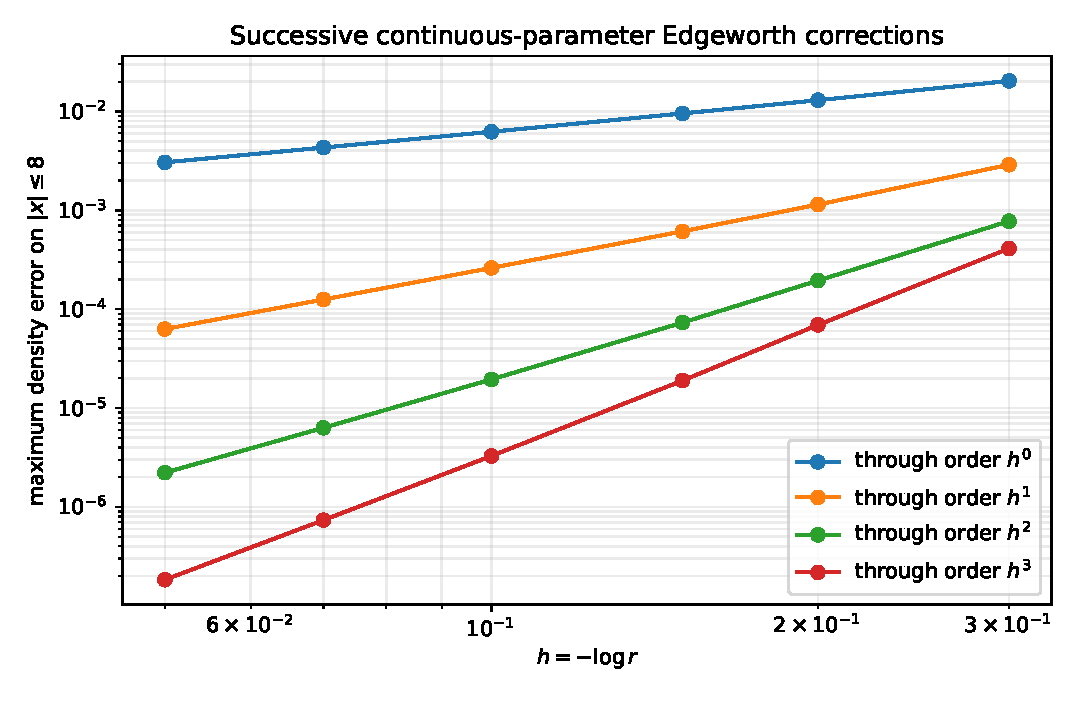
\includegraphics[width=0.88\textwidth]{figures/edgeworth_error_scaling.pdf}
\caption{Log--log error curves for the Gaussian approximation and the first three continuous-parameter Edgeworth corrections.}
\label{fig:edgeworth-scaling}
\end{figure}

\begin{figure}[htbp]
\centering
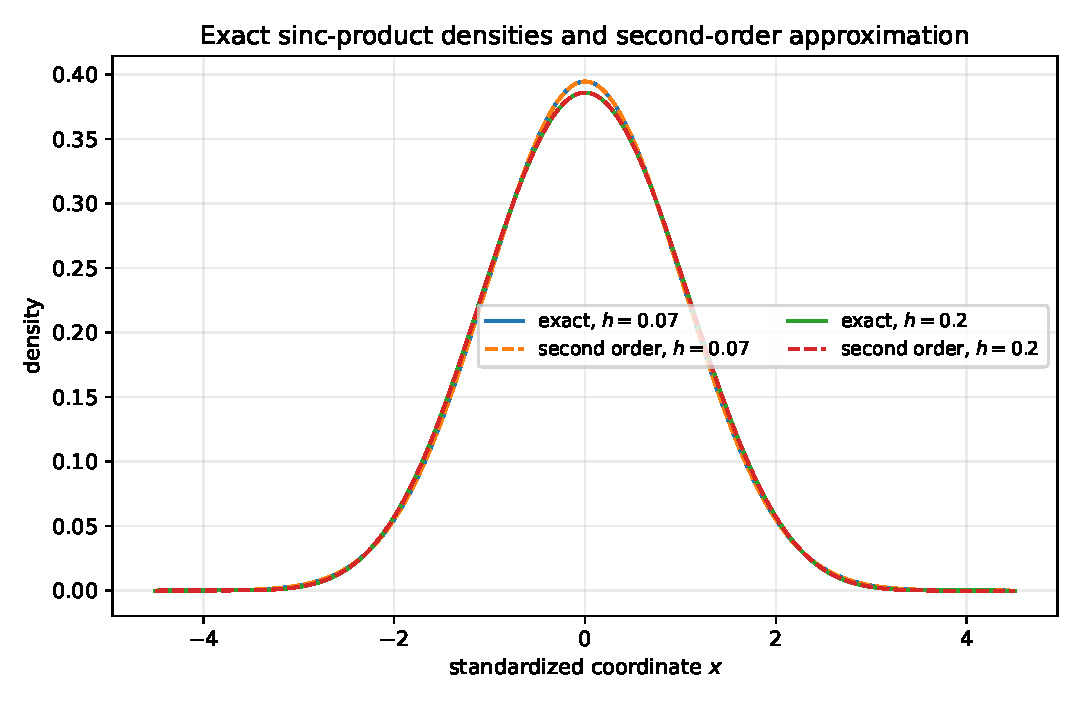
\includegraphics[width=0.88\textwidth]{figures/density_edgeworth_comparison.pdf}
\caption{Exact sinc-product densities and the second-order approximation for two values of \(h\).  The curves are visually indistinguishable near the center at \(h=0.07\).}
\label{fig:density-comparison}
\end{figure}

\subsection{Central quantiles}
At the seven levels \(u\in\{0.05,0.10,0.25,0.50,0.75,0.90,0.95\}\), the maximum errors are:
\begin{table}[htbp]
\centering
\caption{Central quantile errors for the normal, first-order, and second-order Cornish--Fisher approximations.}
\label{tab:quantile-errors}
\begin{tabular}{@{}rrrr@{}}
\toprule
$h$ & Gaussian quantile & first order & second order\\
\midrule
$0.30$ & $3.0365\times 10^{-2}$ & $4.6160\times 10^{-3}$ & $2.2050\times 10^{-3}$\\
$0.20$ & $1.9087\times 10^{-2}$ & $1.9206\times 10^{-3}$ & $4.8685\times 10^{-4}$\\
$0.15$ & $1.3929\times 10^{-2}$ & $1.0540\times 10^{-3}$ & $1.8484\times 10^{-4}$\\
$0.10$ & $9.0414\times 10^{-3}$ & $4.5827\times 10^{-4}$ & $4.9114\times 10^{-5}$\\
$0.07$ & $6.2435\times 10^{-3}$ & $2.2203\times 10^{-4}$ & $1.5399\times 10^{-5}$\\
$0.05$ & $4.4288\times 10^{-3}$ & $1.1264\times 10^{-4}$ & $5.2626\times 10^{-6}$\\
\bottomrule
\end{tabular}

\end{table}
The second-order error behaves consistently with \(\BigO(h^3)\), while the first-order error behaves as \(\BigO(h^2)\).

\subsection{Lambert--\texorpdfstring{$W$}{W} edge check}
The exact parametric rate \eqref{eq:I-parametric} was compared with the edge form \eqref{eq:edge-rate-main}.  Here \(a\) is the saddle and \(\delta=1-y(a)/\sqrt6\).
\begin{table}[htbp]
\centering
\caption{Rapid onset of the Lambert--\(W\) support-edge asymptotic.}
\label{tab:ldp-edge}
\begin{tabular}{@{}rrrr@{}}
\toprule
$a$ & $\delta=1-y/\sqrt6$ & exact $I(y)$ & exact minus Lambert--$W$ form\\
\midrule
$2$ & $0.7023899$ & $0.2810218$ & $-4.246\times 10^{-3}$\\
$3$ & $0.5980804$ & $0.5392933$ & $-3.642\times 10^{-4}$\\
$5$ & $0.4605261$ & $1.0770083$ & $-4.158\times 10^{-6}$\\
$8$ & $0.3465736$ & $1.7997292$ & $-6.640\times 10^{-9}$\\
$10$ & $0.2995732$ & $2.2201676$ & $-9.836\times 10^{-11}$\\
$20$ & $0.1844440$ & $3.8437303$ & $-1.037\times 10^{-19}$\\
\bottomrule
\end{tabular}

\end{table}
The difference is already below \(10^{-10}\) at \(a=10\), despite \(\delta\approx0.30\).  This unusually rapid convergence reflects the exponentially small correction in \eqref{eq:delta-a-exact}.

\begin{figure}[htbp]
\centering
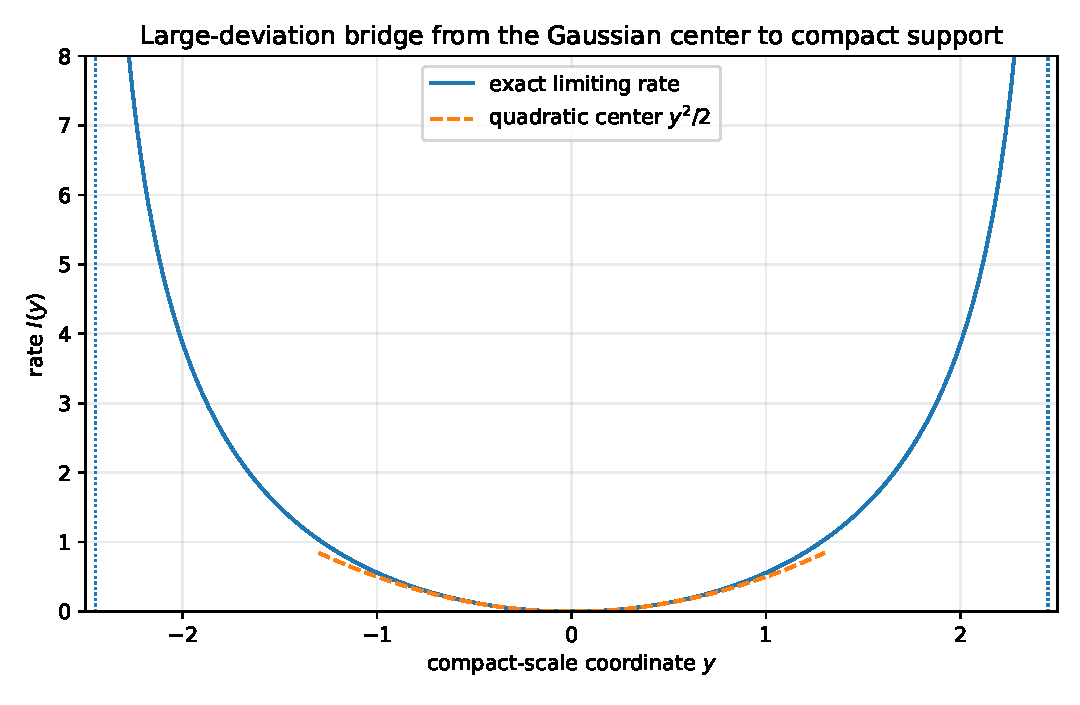
\includegraphics[width=0.88\textwidth]{figures/large_deviation_rate.pdf}
\caption{The exact limiting compact-scale rate.  It is quadratic near the origin and diverges at the limiting support endpoints \(\pm\sqrt6\).}
\label{fig:ldp-rate}
\end{figure}

\section{Conjectures and frontier directions}\label{sec:conjectures}

The theorems above open several directions that are not merely requests for more coefficients.  They concern matching between asymptotic regimes, local symbolic regularity, and arithmetic structure.

\subsection{A matched four-regime asymptotic theory}
\begin{conjecture}[Uniform saddlepoint local large deviations]\label{conj:local-ldp}
For every compact \(K\subset(-\sqrt6,\sqrt6)\), the density of \(Y_h\) has the uniform saddlepoint expansion
\begin{equation}\label{eq:local-ldp-conj}
 f_{Y_h}(y)
 \sim \frac{\exp[-I(y)/h]}{\sqrt{2\pi h\,\Lambda''(s(y))}}
 \sum_{n=0}^{\infty}h^nA_n(y),
 \qquad y\in K,
\end{equation}
where \(s(y)\) is the unique solution of \(\Lambda'(s)=y\), and each \(A_n\) is an explicit differential polynomial in \(\Lambda\).
\end{conjecture}

\begin{conjecture}[Edgeworth--large-deviation matching]\label{conj:matching}
When \(y=\sqrt h\,x\to0\), the saddlepoint expansion \eqref{eq:local-ldp-conj}, re-expanded in \(h\), matches the Bernoulli--Bell--Hermite Edgeworth series term by term.  In the overlap \(1\ll x\ll h^{-1/2}\), it matches the Gaussian moderate-deviation expansion.  This matching is Borel summable in a sector of the complex \(x\)-plane avoiding the images of the nearest sinc zeros.
\end{conjecture}

\begin{conjecture}[Double matching at the compact edge]\label{conj:edge-matching}
There is a two-parameter uniform asymptotic that matches the compact-scale Lambert--\(W\) law \eqref{eq:edge-rate-main} to the fixed-\(r\) endpoint asymptotic with its periodic logarithmic profile.  The crossover occurs when \(\delta\downarrow0\) and \(h\downarrow0\) jointly so that the exact saddle reaches the first geometric lattice scale before the continuum Riemann-sum approximation loses uniformity.
\end{conjecture}

The last conjecture should reveal how the periodic fluctuations at fixed \(r\) disappear in the continuum \(r\uparrow1\) limit.  Poisson summation in the logarithmic index is a promising mechanism: nonzero Fourier modes should be exponentially small in \(1/h\) in the interior but become visible near the edge.

\subsection{Beyond all orders and sinc-zero geometry}
\begin{conjecture}[Resurgent frequency corrections]\label{conj:resurgence}
After optimal truncation of the continuous Edgeworth series, the remainder is controlled by complex saddles associated with the nearest zeros of \(\SincRad(a_hr^nt)\).  Their actions form a geometric lattice, and the Stokes multipliers admit a \(q\)-product description.  The first exponentially small scale is \(\exp(-C/h)\), consistent with the outer-frequency estimate in \Cref{lem:sinc-envelope}.
\end{conjecture}

A practical route is to apply logarithmic Poisson summation to
\[
 \sum_{n\ge0}\log\SincRad(a_h\EulerE^{-nh}t)
\]
and isolate its nonzero dual modes.  This should be the Gaussian-boundary counterpart of the periodic endpoint profiles already present at fixed base.

\subsection{Entropy and information geometry}
The repository conjectures the leading entropy deficit.  \Cref{thm:edgeworth-schwartz} supplies the missing local expansion, but a complete proof still requires global logarithmic control where \(f_h/\phiN\) is small or large.

\begin{conjecture}[Full entropic expansion]\label{conj:entropy}
The relative entropy has a complete expansion
\begin{equation}\label{eq:entropy-series}
 D(\LawOperator(Z_h)\Vert N(0,1))
 \sim \sum_{n\ge2}d_nh^n,
 \qquad d_2=\frac3{100},
\end{equation}
where every \(d_n\) is a finite contraction of Bernoulli-generated Edgeworth coefficients using Hermite orthogonality.  The same holds for Fisher information and for Rényi divergences in a nontrivial interval of orders.
\end{conjecture}

A proof should combine the weighted Edgeworth theorem with a saddlepoint majorant on the scale \(x=O(h^{-1/2})\).  The LDP from \Cref{thm:compact-ldp} provides exactly the missing tail geometry.

\subsection{Local symbolic Carleman spectra}
The global weight in \Cref{thm:carleman-ha} is sharp, but local derivative growth can be much smaller at points whose symbolic orbit repeatedly enters regions where the base profile is tiny.

\begin{problem}[Multifractal local regularity]\label{prob:local-carleman}
For \(a\ge2\) and \(x\) in the symbolic attractor, determine the spectrum of
\begin{equation}\label{eq:local-growth-spectrum}
 \underline\alpha(x)=\liminf_{n\to\infty}\frac{\log\AbsoluteValue{h_a^{(n)}(x)}}{n^2},
 \qquad
 \overline\alpha(x)=\limsup_{n\to\infty}\frac{\log\AbsoluteValue{h_a^{(n)}(x)}}{n^2}.
\end{equation}
Relate the Hausdorff dimensions of level sets to recurrence rates of the digit shift and to thermodynamic pressure.
\end{problem}

\begin{conjecture}[Typical quadratic exponent]\label{conj:typical-carleman}
For the natural Bernoulli measure on the symbolic attractor of \(h_a\),
\[
 \underline\alpha(x)=\overline\alpha(x)=\frac12\log a
\]
for almost every \(x\), while exceptional recurrent orbits realize a nontrivial interval of lower subleading exponents.
\end{conjecture}

\subsection{The overlapping phase \texorpdfstring{$1<a<2$}{1<a<2}}
The exact norm formula uses disjoint cylinder supports and therefore stops at \(a=2\).  Fourier methods still give
\[
 \log\Norm{h_a^{(n)}}_\infty\le\frac{\log a}{2}n^2+\BigO_a(n\log n).
\]

\begin{conjecture}[Sharp quadratic exponent under overlap]\label{conj:overlap-growth}
For every \(1<a<2\),
\begin{equation}\label{eq:overlap-conj}
 \lim_{n\to\infty}\frac1{n^2}\log\Norm{h_a^{(n)}}_\infty
 =\frac12\log a.
\end{equation}
The subleading term changes at parameters with exceptional Bernoulli-convolution overlap, and may encode arithmetic properties of \(a\).
\end{conjecture}

This conjecture would extend the quadratic \(q\)-Gevrey classification through the entire smooth geometric family, while leaving room for arithmetic phase transitions in the \(n\log n\) or linear term.

\subsection{Arithmetic and Thue--Morse directions}
\begin{conjecture}[Cumulant-coefficient denominators]\label{conj:cumulant-denominators}
After the natural normalization by \((2m)!\), the coefficients in the \(h\)-expansion \eqref{eq:lambda-bell} have denominators controlled by von Staudt--Clausen primes from the Bernoulli numbers and by the divisors of \(m^{2k}-m\).  There is a finite-prime valuation formula compatible with the dyadic arithmetic of \(F(2^{-n})\).
\end{conjecture}

\begin{problem}[Automatic-sequence Edgeworth analogs]
Replace the uniform digits in \eqref{eq:Xr-def} by signed or block-dependent digits generated by Thue--Morse and other automatic sequences.  Determine when a Gaussian boundary survives, how automatic cancellations alter the first nonzero cumulant, and whether the resulting Edgeworth polynomials inherit finite-kernel recurrences.
\end{problem}

\begin{problem}[Legendre--Hermite contraction]
The repository develops compact-support Legendre and Jacobi expansions, whereas the Gaussian boundary naturally selects the Hermite basis.  Determine a joint limit in the polynomial degree and in \(h\downarrow0\) under which the appropriately rescaled Legendre/Jacobi coefficients contract to the Bernoulli--Bell--Hermite Edgeworth coefficients.  A successful contraction formula would connect the global compact-support spectral theory to the local Gaussian asymptotic theory without passing through pointwise Fourier inversion.
\end{problem}

\subsection{Formalization targets}
The analytic arguments naturally split into reusable lemmas suitable for Lean or another proof assistant:
\begin{enumerate}
\item exact cumulant algebra and hyperbolic simplification;
\item the global sinc envelope and geometric power-sum bounds;
\item weighted Fourier inversion from \(W^{K,1}\) estimates;
\item the Riemann-sum limit for \(\Lambda_h\);
\item strict convexity and Legendre duality;
\item the Mellin finite-part computation of \(\mathfrak C\);
\item the Carleman ratio test for the exact norm sequence.
\end{enumerate}
The most delicate formalization component is the all-orders bookkeeping in \Cref{thm:edgeworth-schwartz}; encoding the weight \(w(\bm k)\) as a graded finite-support map should make the Bell combinatorics manageable.

\section{Promising research program}\label{sec:program}

A productive sequence of projects, ordered by mathematical dependency rather than by perceived difficulty, is:

\begin{enumerate}[label=\textbf{P\arabic*.}]
\item \textbf{Local saddlepoint theorem.}  Prove \Cref{conj:local-ldp} by complex Fourier inversion around the unique imaginary saddle.  Establish uniformity on compact subsets of the open limiting support.
\item \textbf{Central matching.}  Expand the saddlepoint coefficients at \(y=0\) and identify them combinatorially with the Bernoulli--Bell--Hermite coefficients of \Cref{thm:edgeworth-schwartz}.
\item \textbf{Entropic CLT with coefficients.}  Combine weighted central control and the compact-scale LDP to prove \Cref{conj:entropy}, first through \(h^3\), then to all orders.
\item \textbf{Logarithmic Poisson modes.}  Derive the exponentially small correction between the geometric Riemann sum and its continuum integral.  Identify the first dual mode and its Stokes geometry.
\item \textbf{Edge crossover.}  Construct the double-scaling asymptotic of \Cref{conj:edge-matching}, retaining the fixed-base periodic phase until it is exponentially suppressed.
\item \textbf{Overlapping quadratic regularity.}  Prove \eqref{eq:overlap-conj}; investigate whether Pisot, Salem, or exact-overlap parameters alter subleading derivative growth.
\item \textbf{Local Carleman thermodynamics.}  Translate the exact symbolic derivative formula into a subadditive pressure problem and compute the multifractal spectrum in \Cref{prob:local-carleman}.
\item \textbf{Arithmetic coefficient package.}  Implement exact Bernoulli--Bell coefficient generation, valuation analysis, and conjecture discovery for \eqref{eq:lambda-bell} and the quantile polynomials.
\item \textbf{Legendre--Hermite contraction.}  Derive the double-scaling limit in the preceding problem and use it to transfer spectral estimates between compact-support and Gaussian-boundary regimes.
\end{enumerate}

The first five projects form a single asymptotic arc from the Gaussian center to the fixed-parameter endpoint.  Projects six through eight exploit the independent but structurally parallel quadratic growth appearing in derivatives, \(q\)-products, and arithmetic denominators; the ninth connects the repository's orthogonal-polynomial and Gaussian asymptotic languages.

\section{Conclusion}
The geometric-uniform deformation turns the Fabius/Rvachev pair into a parameterized laboratory in which several asymptotic languages coexist.  The exact cumulants make Bernoulli numbers primary; exponential composition turns them into Bell polynomials; Fourier inversion turns Bell monomials into Hermite corrections; inversion of the CDF produces Cornish--Fisher polynomials; rescaling to the compact support produces a G\"artner--Ellis rate; and approaching that support edge produces the lower Lambert branch and a Stieltjes constant.  Independently, the Thue--Morse derivative hierarchy produces an exact quadratic-exponential Carleman weight, whose Legendre dual is the log-Gaussian Fourier envelope.

The central result is therefore not only a missing Edgeworth estimate.  It is a bridge between the repository's probability, \(q\)-series, inverse-function, Lambert--\(W\), Bernoulli/Bell, Fourier-product, and automatic-sequence components.  The large-deviation and quadratic \(q\)-Gevrey theorems show that the same geometric scaling controls both the parameter boundary \(r\uparrow1\) and the derivative order \(n\to\infty\), but through different Legendre transforms.  This duality appears to be a fertile organizing principle for the next phase of the Fabius--Rvachev program.

\appendix

\section{Explicit Hermite polynomials and third-order formulas}\label{app:hermite}
The probabilists' Hermite polynomials used above begin
\begin{align*}
H_3(x)&=x^3-3x,\\
H_4(x)&=x^4-6x^2+3,\\
H_5(x)&=x^5-10x^3+15x,\\
H_6(x)&=x^6-15x^4+45x^2-15,\\
H_7(x)&=x^7-21x^5+105x^3-105x,\\
H_8(x)&=x^8-28x^6+210x^4-420x^2+105.
\end{align*}
The third-order CDF expansion obtained by integrating \eqref{eq:edgeworth-three-orders} is
\begin{align}\label{eq:cdf-third-order}
F_h(x)=\PhiN(x)+\phiN(x)\Bigg[&\frac h{20}H_3(x)
-h^2\left(\frac4{315}H_5(x)+\frac1{800}H_7(x)\right)\notag\\
&+h^3\left(-\frac1{60}H_3(x)+\frac3{700}H_7(x)
+\frac1{1575}H_9(x)+\frac1{48000}H_{11}(x)\right)\Bigg]\notag\\
&+\BigO_{\mathrm{weighted}}(h^4).
\end{align}

\section{A coefficient-extraction form of the full Edgeworth series}\label{app:coefficient}
Treat \(h\) as a formal variable and write the cumulant expansions from \Cref{thm:cumulant-bell} as
\[
 \lambda_{2m}(h)=\sum_{n\ge m-1}\lambda_{2m,n}h^n.
\]
Then the coefficient of \(h^N\) in the density expansion is
\begin{equation}\label{eq:coefficient-extraction}
 P_N(x)=[h^N]\exp_{\mathcal H}\!\left(
 \sum_{m\ge2}\frac{\lambda_{2m}(h)}{(2m)!}\,H_{2m}\right),
\end{equation}
where \(\exp_{\mathcal H}\) means that multiplication is performed before replacing \((\ImaginaryUnit t)^{2k}\) by \(H_{2k}(x)\).  More explicitly,
\begin{equation}\label{eq:PN-explicit}
 P_N(x)=
 \sum_{\substack{k_2,k_3,\ldots\ge0\\
 n_{m,j}\ge0\\
 \sum_{m,j}jn_{m,j}=N\\
 \sum_jn_{m,j}=k_m}}
 H_{2\sum_mmk_m}(x)
 \prod_{m\ge2}\frac1{k_m!(2m)!^{k_m}}
 \frac{k_m!}{\prod_jn_{m,j}!}
 \prod_j\lambda_{2m,j}^{n_{m,j}}.
\end{equation}
Only finitely many indices occur for each \(N\), because \(\lambda_{2m,j}=0\) for \(j<m-1\).  Formula \eqref{eq:PN-explicit} is suitable for exact symbolic generation.

\section{Large-deviation series derivation}\label{app:ldp-series}
From \eqref{eq:log-sinh},
\begin{align*}
\Lambda(s)
&=\int_0^1\sum_{k\ge1}c_k(\sqrt6\,su)^{2k}\frac{\Differential u}{u}\\
&=\sum_{k\ge1}\frac{c_k6^k}{2k}s^{2k}.
\end{align*}
This yields \eqref{eq:Lambda-series}.  To compute \(I\), solve \(y=\Lambda'(s)\) recursively:
\begin{equation}\label{eq:s-of-y}
 s(y)=y+\frac15y^3+\frac{23}{525}y^5+\frac{22}{2625}y^7
 +\frac{821}{606375}y^9+\BigO(y^{11}).
\end{equation}
Substitution into \(I(y)=ys(y)-\Lambda(s(y))\) gives \eqref{eq:I-center-series}.

\section{Reproducibility and files}\label{app:repro}
The accompanying archive has the following layout:
\begin{lstlisting}
fabius_frontier_report.tex
fabius_frontier_report.pdf
README.md
requirements.txt
MANIFEST.txt
SHA256SUMS
numerics/fabius_q_edgeworth.py
numerics/README.md
data/edgeworth_errors.csv
  data/edgeworth_table.tex
data/quantile_errors.csv
  data/quantile_table.tex
data/large_deviation_edge.csv
  data/ldp_edge_table.tex
figures/edgeworth_error_scaling.{pdf,png}
figures/density_edgeworth_comparison.{pdf,png}
figures/large_deviation_rate.{pdf,png}
\end{lstlisting}
To install the numerical dependencies and regenerate every CSV table, LaTeX table, and figure:
\begin{lstlisting}[language=bash]
python -m pip install -r requirements.txt
python numerics/fabius_q_edgeworth.py --output-dir .
\end{lstlisting}
To rebuild the report:
\begin{lstlisting}[language=bash]
latexmk -pdf -interaction=nonstopmode -halt-on-error fabius_frontier_report.tex
\end{lstlisting}

\section{Repository source inventory used in the audit}\label{app:inventory}
The main live source files and inventory documents consulted were (each canonical file is in its same-named directory):
\begin{itemize}
\item \path{FabiusFunction_Mathematical_Glossary.tex};
\item \path{Fabius_Function_and_Rvachev_Up.tex};
\item \path{Non_Elementarity_of_the_Fabius_Function.tex};
\item \path{fabius_lean_walkthrough.tex};
\item \path{semi-formalized-research-frontiers.tex};
\item the draft \texttt{MANIFEST.md}, with raw inspection of the Gaussian-boundary report, the consolidated exponents-and-\(q\)-series volume, the general-base atomic-function chapters, inverse-\(q\) reports, Fourier-decay audits, and candidate overlap documents;
\item imported LaTeX sources for Arias de Reyna's compact-support and arithmetic papers, Allouche--Shallit's Thue--Morse survey, the lacunary-product papers, and the Thue--Morse Dirichlet-series paper;
\item the historical archive README and category inventories.
\end{itemize}
The public path is
\begin{center}
\url{https://github.com/VladimirReshetnikov/ProveIt/tree/main/Analysis/FabiusFunction/docs}.
\end{center}

\begin{thebibliography}{99}

\bibitem{Arias1982}
J.~Arias de Reyna,
\newblock \emph{An infinitely differentiable function with compact support: Definition and properties},
\newblock English translation of Rev. Real Acad. Cienc. Exact. F\'is. Natur. Madrid \textbf{76} (1982), 21--38,
\newblock arXiv:1702.05442.

\bibitem{Arias2017}
J.~Arias de Reyna,
\newblock \emph{Arithmetic of the Fabius function},
\newblock arXiv:1702.06487 (2017).

\bibitem{AlloucheShallit}
J.-P.~Allouche and J.~Shallit,
\newblock \emph{The ubiquitous Prouhet--Thue--Morse sequence},
\newblock in Sequences and Their Applications, Springer, 1999, pp.~1--16.

\bibitem{AistleitnerParametric}
C.~Aistleitner, R.~Hofer, and G.~Larcher,
\newblock \emph{On parametric Thue--Morse sequences and lacunary trigonometric products},
\newblock arXiv:1502.06738.

\bibitem{AistleitnerEvil}
C.~Aistleitner, R.~Hofer, and G.~Larcher,
\newblock \emph{On evil Kronecker sequences and lacunary trigonometric products},
\newblock Ann. Inst. Fourier \textbf{67} (2017), 637--687.

\bibitem{BhattacharyaRao}
R.~N.~Bhattacharya and R.~Rao,
\newblock \emph{Normal Approximation and Asymptotic Expansions},
\newblock SIAM, 2010 reprint.

\bibitem{CorlessLambertW}
R.~M.~Corless, G.~H.~Gonnet, D.~E.~G.~Hare, D.~J.~Jeffrey, and D.~E.~Knuth,
\newblock \emph{On the Lambert W function},
\newblock Adv. Comput. Math. \textbf{5} (1996), 329--359.

\bibitem{DemboZeitouni}
A.~Dembo and O.~Zeitouni,
\newblock \emph{Large Deviations Techniques and Applications},
\newblock 2nd ed., Springer, 1998; corrected printing 2010.

\bibitem{Fabius1966}
J.~Fabius,
\newblock \emph{A probabilistic example of a nowhere analytic \(C^\infty\)-function},
\newblock Z. Wahrscheinlichkeitstheorie verw. Gebiete \textbf{5} (1966), 173--174.

\bibitem{Haugland}
J.~K.~Haugland,
\newblock \emph{Evaluating the Fabius function},
\newblock arXiv:1609.07999 (2016).

\bibitem{JessenWintner}
B.~Jessen and A.~Wintner,
\newblock \emph{Distribution functions and the Riemann zeta function},
\newblock Trans. Amer. Math. Soc. \textbf{38} (1935), 48--88.

\bibitem{Komatsu}
H.~Komatsu,
\newblock \emph{Ultradistributions I: Structure theorems and a characterization},
\newblock J. Fac. Sci. Univ. Tokyo Sect. IA Math. \textbf{20} (1973), 25--105.

\bibitem{Petrov}
V.~V.~Petrov,
\newblock \emph{Sums of Independent Random Variables},
\newblock Springer, 1975.

\bibitem{RepoPrimary}
V.~Reshetnikov et al.,
\newblock \emph{The Fabius function and Rvachev's up function}, living LaTeX exposition,
\newblock \repo\ repository, accessed 30 August 2026.

\bibitem{RepoFrontier}
V.~Reshetnikov et al.,
\newblock \emph{Semi-formalized research frontiers for the Fabius and Rvachev functions}, living LaTeX frontier volume,
\newblock \repo\ repository, accessed 30 August 2026.

\bibitem{RepoGaussian}
V.~Reshetnikov et al.,
\newblock \emph{Fabius--Rvachev frontier report}, Gaussian-boundary and geometric-parameter draft,
\newblock \repo\ repository, accessed 30 August 2026.

\bibitem{RepoExponents}
V.~Reshetnikov et al.,
\newblock \emph{Exponents and \(q\)-series frontiers}, consolidated draft volume,
\newblock \repo\ repository, accessed 30 August 2026.

\bibitem{Toth}
L.~T\'oth,
\newblock \emph{Linear combinations of Dirichlet series associated with the Thue--Morse sequence},
\newblock arXiv:2211.13570 (2022).

\end{thebibliography}

\end{document}
